\documentclass[11pt, a4paper]{article}

\usepackage{amsmath}
\usepackage{commath}
\usepackage{url}
\usepackage{cite}
\usepackage{color}
\usepackage{multirow}
\usepackage[margin=1.25in]{geometry}
\usepackage{graphicx}
\usepackage[T1]{fontenc}
\usepackage[utf8]{inputenc}
\usepackage{authblk}
\graphicspath{{./graphics/}}

\newcommand\T{\rule{0pt}{2.6ex}}       % Top strut
\newcommand\B{\rule[-1.2ex]{0pt}{0pt}} % Bottom strut

\title{GlueX DIRC Writeup}

\author[1]{M.~Patsyuk\thanks{mpatsyuk@mit.edu}}
\author[2]{R.~Dzhydaglo\thanks{r.dzhygadlo@gsi.de}}
\affil[1]{\small{Massachusetts Institute of Technology, Cambridge, USA}}
\affil[2]{\small{GSI Helmholtzzentrum f{\"u}r Schwerionenforschung GmbH, Darmstadt, Germany}}

\date{\vspace{-5ex}}

\begin{document}

\maketitle

\begin{abstract}
This note presents a description of the GlueX DIRC simulation and reconstruction software. The geometrical algorithm, based on the one developed for the BABAR DIRC, can be used as the baseline recontruction method for the start of the DIRC operation in 2018. The time imaging reconstruction has potential for better performance but requires additional development work and a time resolution of (how much?) ns per photon. The KDE-based method is planned to be used for the tracks where the PID is not clear after the baseline reconstruction is run (on average, the resolution for the KDE-based method is 30{\%} better than for the geometrical reconstruction).
\end{abstract}

\vspace{5 cm}
%\centering{
Version 1.0

\newpage

\tableofcontents

\newpage

\section{Detector design}

In this chapter we will describe the purpose and general design of the GlueX DIRC.

The GlueX DIRC detector~\cite{dirc} is designed to improve particle identification (PID) capabilities in the forward region of the GlueX~\cite{gluex1, gluex2} detector located in Hall D at Jefferson Lab. The baseline PID in the forward region of the GlueX detector is done by a Time-Of-Flight (TOF) wall, which separates kaons from pions up to momentum around 2 GeV/c. The GlueX DIRC is designed to provide clean separation between kaons and pions with at least three standard deviations for momenta up to 4 GeV/c.

\begin{figure}[!htb]
\centering
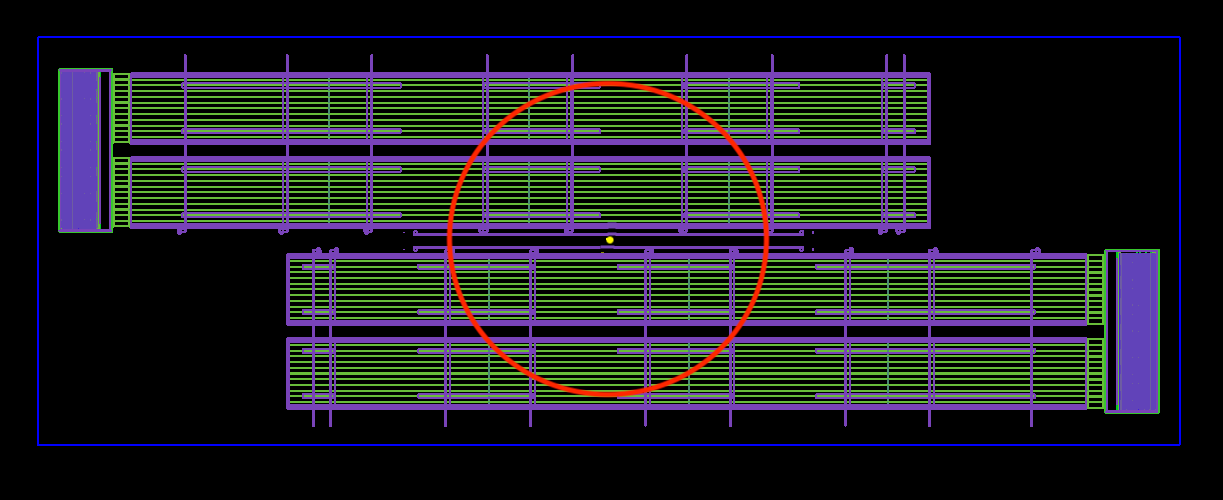
\includegraphics[width=0.9\textwidth]{pics/sim1.png}
\caption{\label{pic:sim}
The view (downstream the beam) of the GlueX DIRC optical system (from the simulation). The beam going into the page is shown in yellow. The red circle shows the polar angle acceptance ($11^{\circ}$ degrees).
The blue box around the detector is the auxiliary volume \texttt{DIRC} containing all the DIRC components, which can be activated/deactivated in the Hall D geometry (see Sec.~\ref{sec:sim}) to insert/remove the GlueX DIRC to/from the GlueX DIRC detector simulation.}
\end{figure}

The GlueX DIRC forms a wall about 4 m away from the target directly upstream of the TOF detector. The DIRC consists of four BABAR DIRC~\cite{bdirc1} bar boxes and covers the polar angle range from $2^{\circ}$ to $11^{\circ}$ (see Fig.~\ref{pic:sim}). Two bar boxes located above the beam line are attached to a photon camera located to the left of the beam. Another pair of the bar boxes covering the acceptance below the beam line is attached to the second photon camera located to the right of the beam. The support structure of the DIRC (shown in Fig.~\ref{pic:support}) allows the pairs of bar boxes to swap out of the active area of the detector (see Fig.~\ref{pic:retracted}) for experiments requiring minimal material budget in front of the forward calorimeter.

The BABAR DIRC bar boxes number 0, 1, 10, 11 (out of twelve) were designated for the GlueX DIRC. They were transported by a truck from SLAC, where all the bar boxes had been stored after the BABAR experiment was disassembled. The structure of a bar box is shown in Fig.~\ref{pic:bbox}. It is an isolated unit with $12$ long radiator bars ($35 \times 17.25 \times 4900 $ mm$^3$) inside. A small wedge is attached to the readout end of each radiator. Bar boxes have to be used without modifications, which means that the small wedges have to stay in the optical system of the GlueX DIRC.

\begin{figure}[h]
\centering
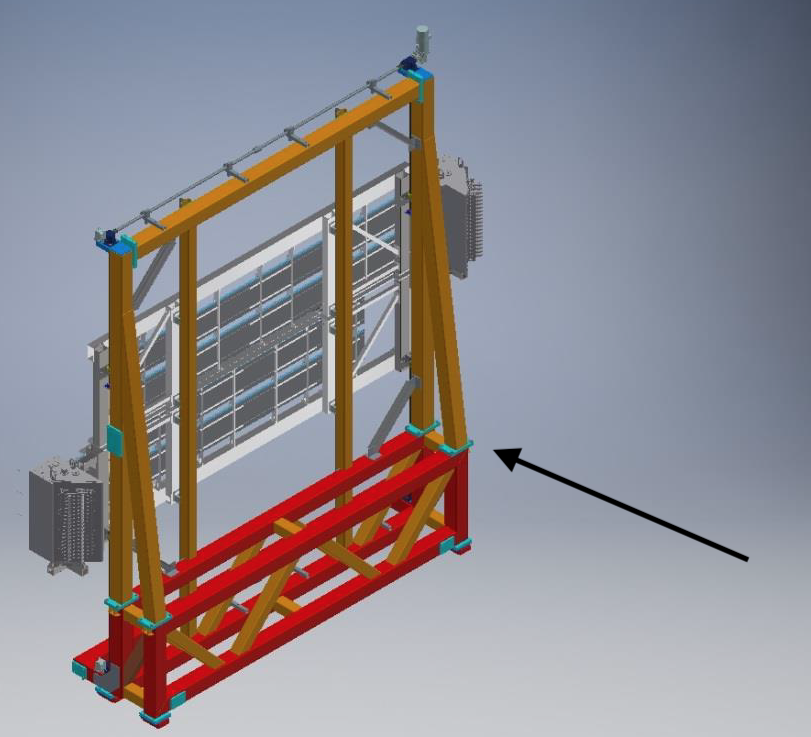
\includegraphics[width=0.6\textwidth]{pics/support.png} 
\caption{\label{pic:support}} A technical drawing of the support structure with the DIRC optical system installed. The bar boxes slide up and down within the orange frame. The beam is coming from the right.
\end{figure}

\begin{figure}[!h]
\centering
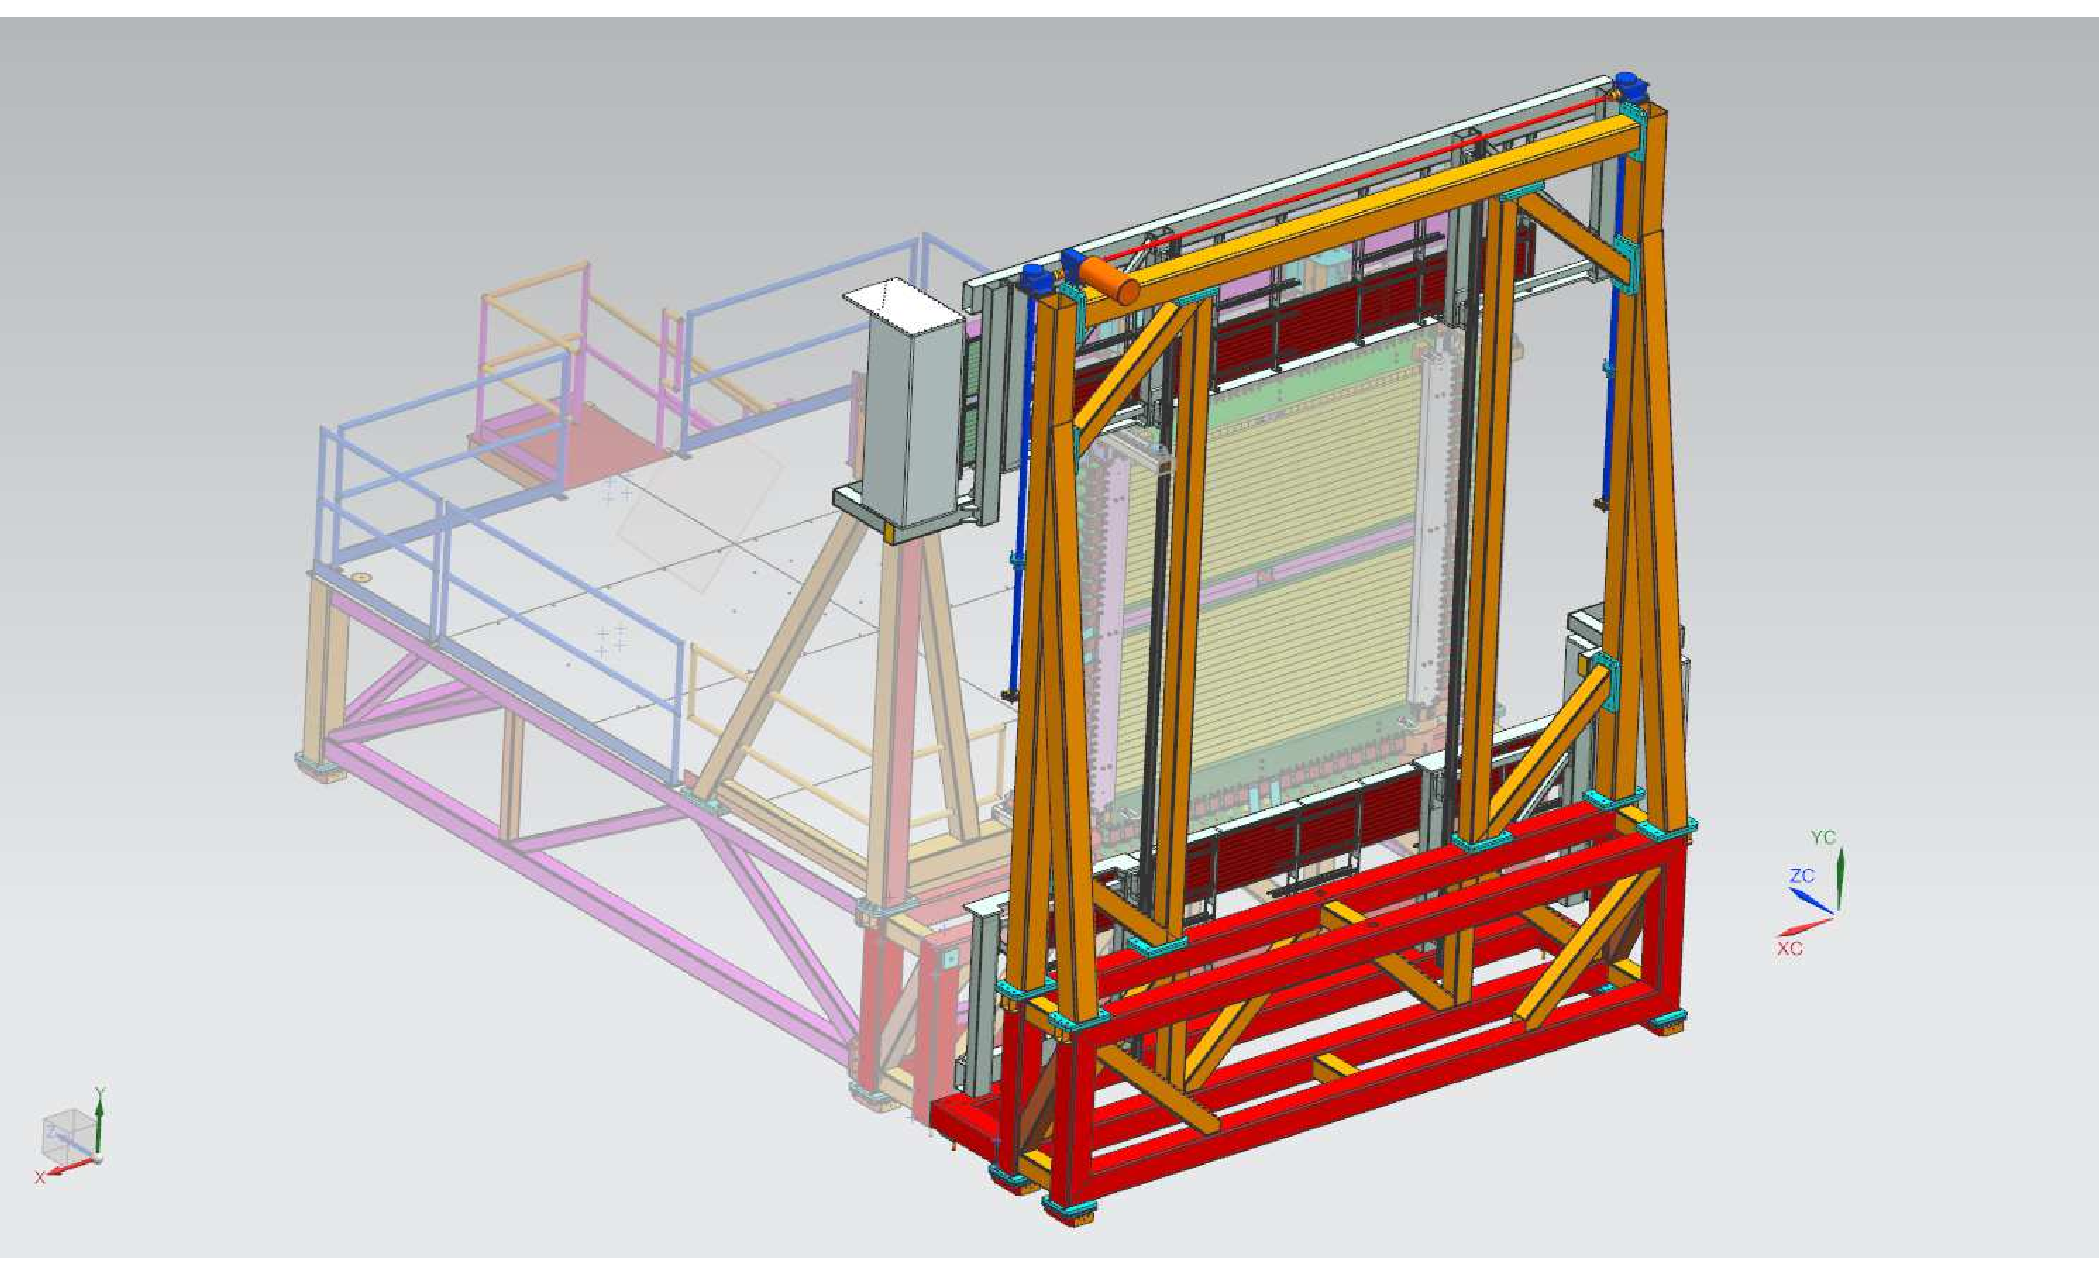
\includegraphics[width=0.9\textwidth]{pics/Full_Assy_Iso-retracted.pdf}
\caption{\label{pic:retracted}} A technical drawing of the support structure with the DIRC retracted. The beam is coming from the right. The active area of the Forward Calorimeter is shown behind the DIRC. The platform is for the other forward GlueX detectors.
\end{figure}

\begin{figure}[!h]
\centering
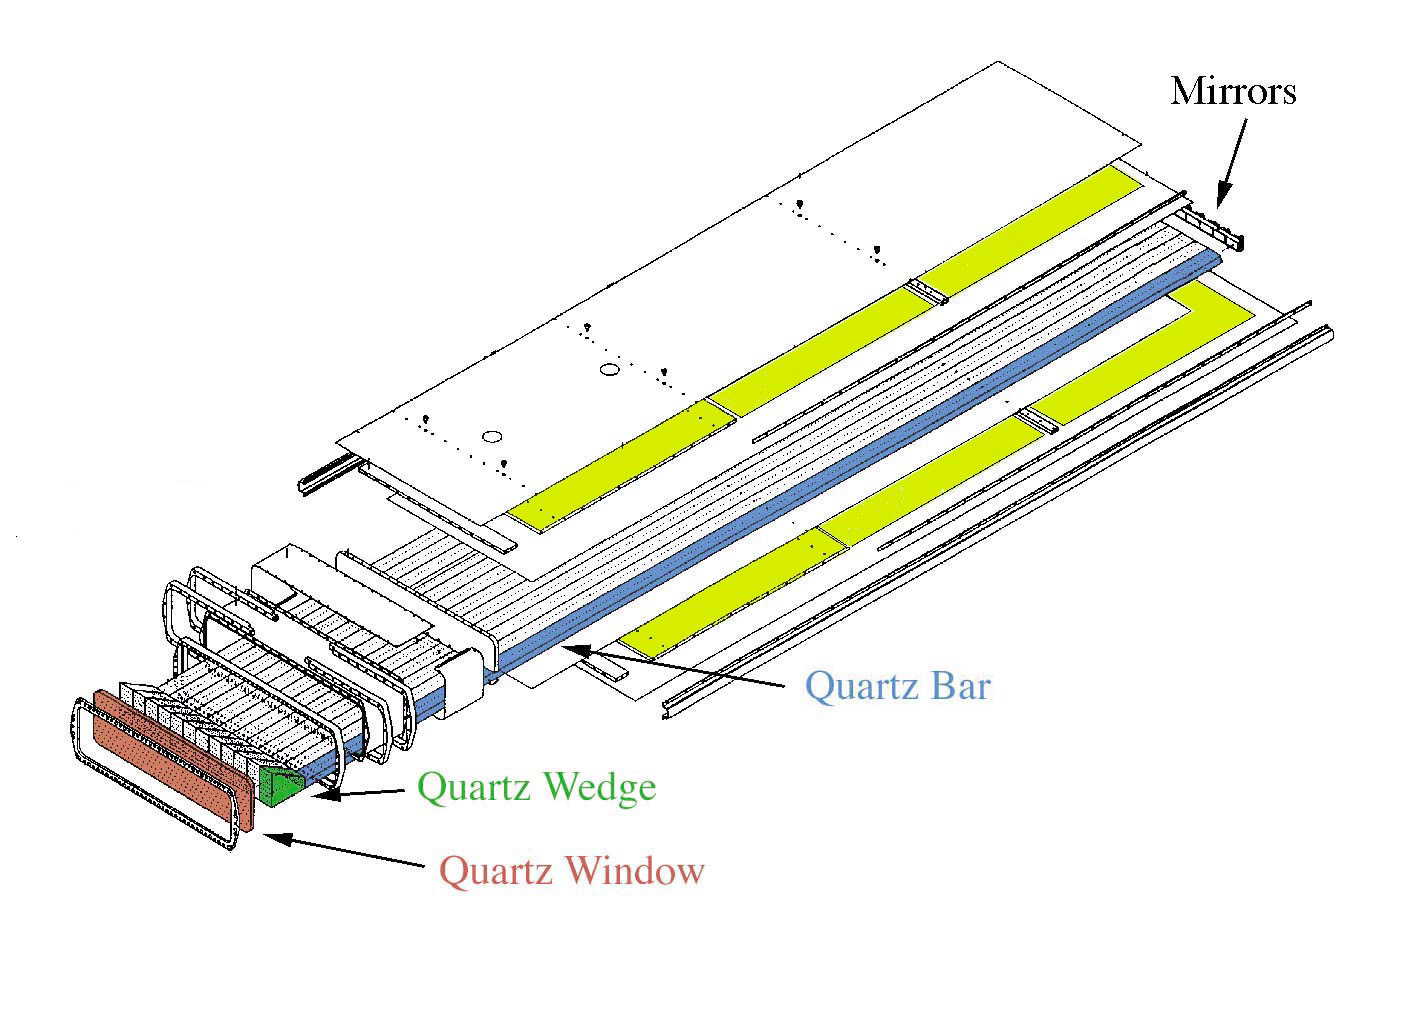
\includegraphics[width=0.8\textwidth]{pics/bab_col.jpg}
\caption{\label{pic:bbox} Schematic of the BABAR DIRC bar box assembly. The single radiator bar is highlighted in blue, the small wedge -- in green.}
\end{figure}

The design of the photon camera is based on the SuperB FDIRC\footnote{FDIRC was designed to be the successor of the BABAR DIRC, but the the SuperB project was cancelled in 2012.} prototype~\cite{fdirc} developed at SLAC. Figure~\ref{pic:ob} shows both cameras. The FDIRC photon camera design was based on compact focussing blocks made of fused silica, one for each bar box in a barrel. For the GlueX DIRC planar orientation one common camera, filled with distilled water, are used for two bar boxes together. This design with wider cameras (the width is $983$ mm) reduces the fraction of photons reflecting off the sides, simplifying the hit pattern and removing ambiguities in the reconstruction (reconstruction details see in Sec.~\ref{sec:gr} and Sec.~\ref{sec:ti}). Another important modification of the photon camera is the approximation of the cylindrical mirror by a set of three flat segments for simplicity in alignment and construction. The photosensors are coupled to the quartz window using silicone pads, which helps to avoid photon loss between the window of the photon camera and photosensors. 

\begin{figure}[!h]
\begin{center}
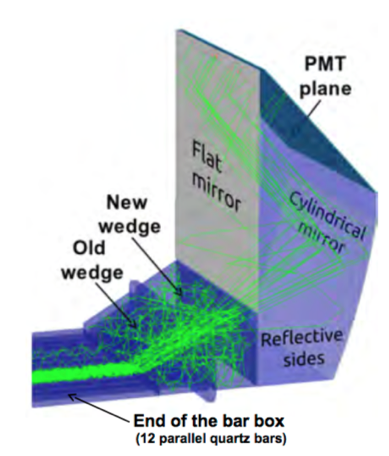
\includegraphics[width=0.3\textwidth]{pics/superB.png} \hspace{0.5cm} 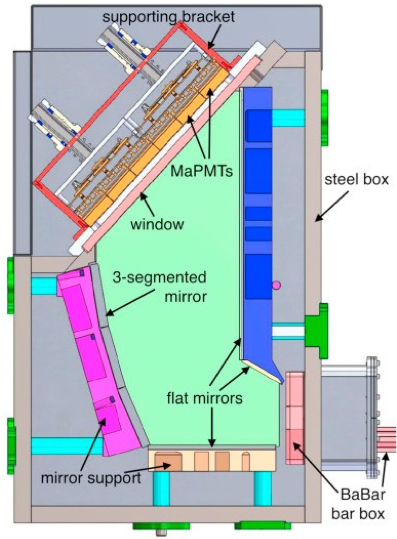
\includegraphics[width=0.4\textwidth]{pics/pc.png}
\end{center}
\caption{\label{pic:ob} Photon camera for the SuperB (left) and for the GlueX DIRC (right). The photon camera for the GlueX DIRC is a steel tank filled with distilled water with immersed mirrors to resemble the shape of the photon camera for the SuperB FDIRC.}
\end{figure}

The GlueX DIRC is read out by an array of Hamamatsu H12700 Multi-Anode PMTs (MaPMTs). The electronics boards are the same as for the CLAS12 RICH in Hall B. They are compatible with the generic JLab DAQ systems.

\section{Simulation}
\label{sec:sim}

This chapter describes the details of the detector simulation, including the geometry, materials, and physical processes, which need to be taken into account. 

\subsection{Geometry}

The simulation of the GlueX DIRC detector within the GlueX software is based on Geant4 (\texttt{hdgeant4} package). The GlueX DIRC in simulation is defined by the geometry description (located in  \texttt{hdds/DIRC{\_}HDDS.xml}) and the functionality of the sensitive elements (described in \texttt{hdgeant4/src/GlueXSensitiveDetectorDIRC} class). 

The detector geometry is an important part of the detector simulation. It should represent all main features of the detector and contain all the elements responsible for the detector response. At the same time it should be simple and contain as few geometrical constituents as possible to keep the simulation fast. The GlueX DIRC geometry is shown in Fig.~\ref{pic:dirc}. Each volume is defined by its shape and material (the list of materials for the GlueX simulation is in \texttt{hdds/Material{\_}HDDS.xml}). 

\vspace{0.5cm}
Some basic rules for constructing a Geant geometry:
\begin{itemize}
\item Geant supports hierarchy, when daughter-volumes are located inside of a mother-volume.  Here one should make sure the daughter-volumes are completely within the mother volume. In case some part of a daughter-volume sticks out from the mother volume, a so-called ''overlap'' occurs. Such overlaps should be avoided. To check for overlaps, one has to uncomment the line \texttt{CHECK{\_}OVERLAPS{\_}MM} in the \texttt{GNUmakefile} in the top directory of the \texttt{hdgeant4} project and then recompile the \texttt{hdgeant4} project (for this do \texttt{touch src/HddsG4Builder.cc} and then \texttt{make} -- this only rebuilds classes that need to change)
\item The coordinates of the daughter-volume are set in the local coordinate system of the mother volume. The origin is at the center of the mother volume, if it is a box, and should be looked up in the Geant4 manuals otherwise
\item When creating a volume, e.g.
%\vspace{0.5cm}
\begin{center}
 \texttt{<box name="DCMV" X{\_}Y{\_}Z="560.0 250.0 150.0" material="OpticalAir" />} 
\end{center}
%\vspace{0.5cm}
\noindent its full (not half) dimenstions should be set. Here the box has dimensions of 560 cm x 250 cm x 150 cm.
\item Volumes can be grouped in assemblies called compositions. Inside a composition volumes are located with respect to the center of the composition. When the composition is placed inside the mother-volume, its center is placed with respect to the center of the mother-volume.
\end{itemize}

\begin{figure}[!h]
\centering
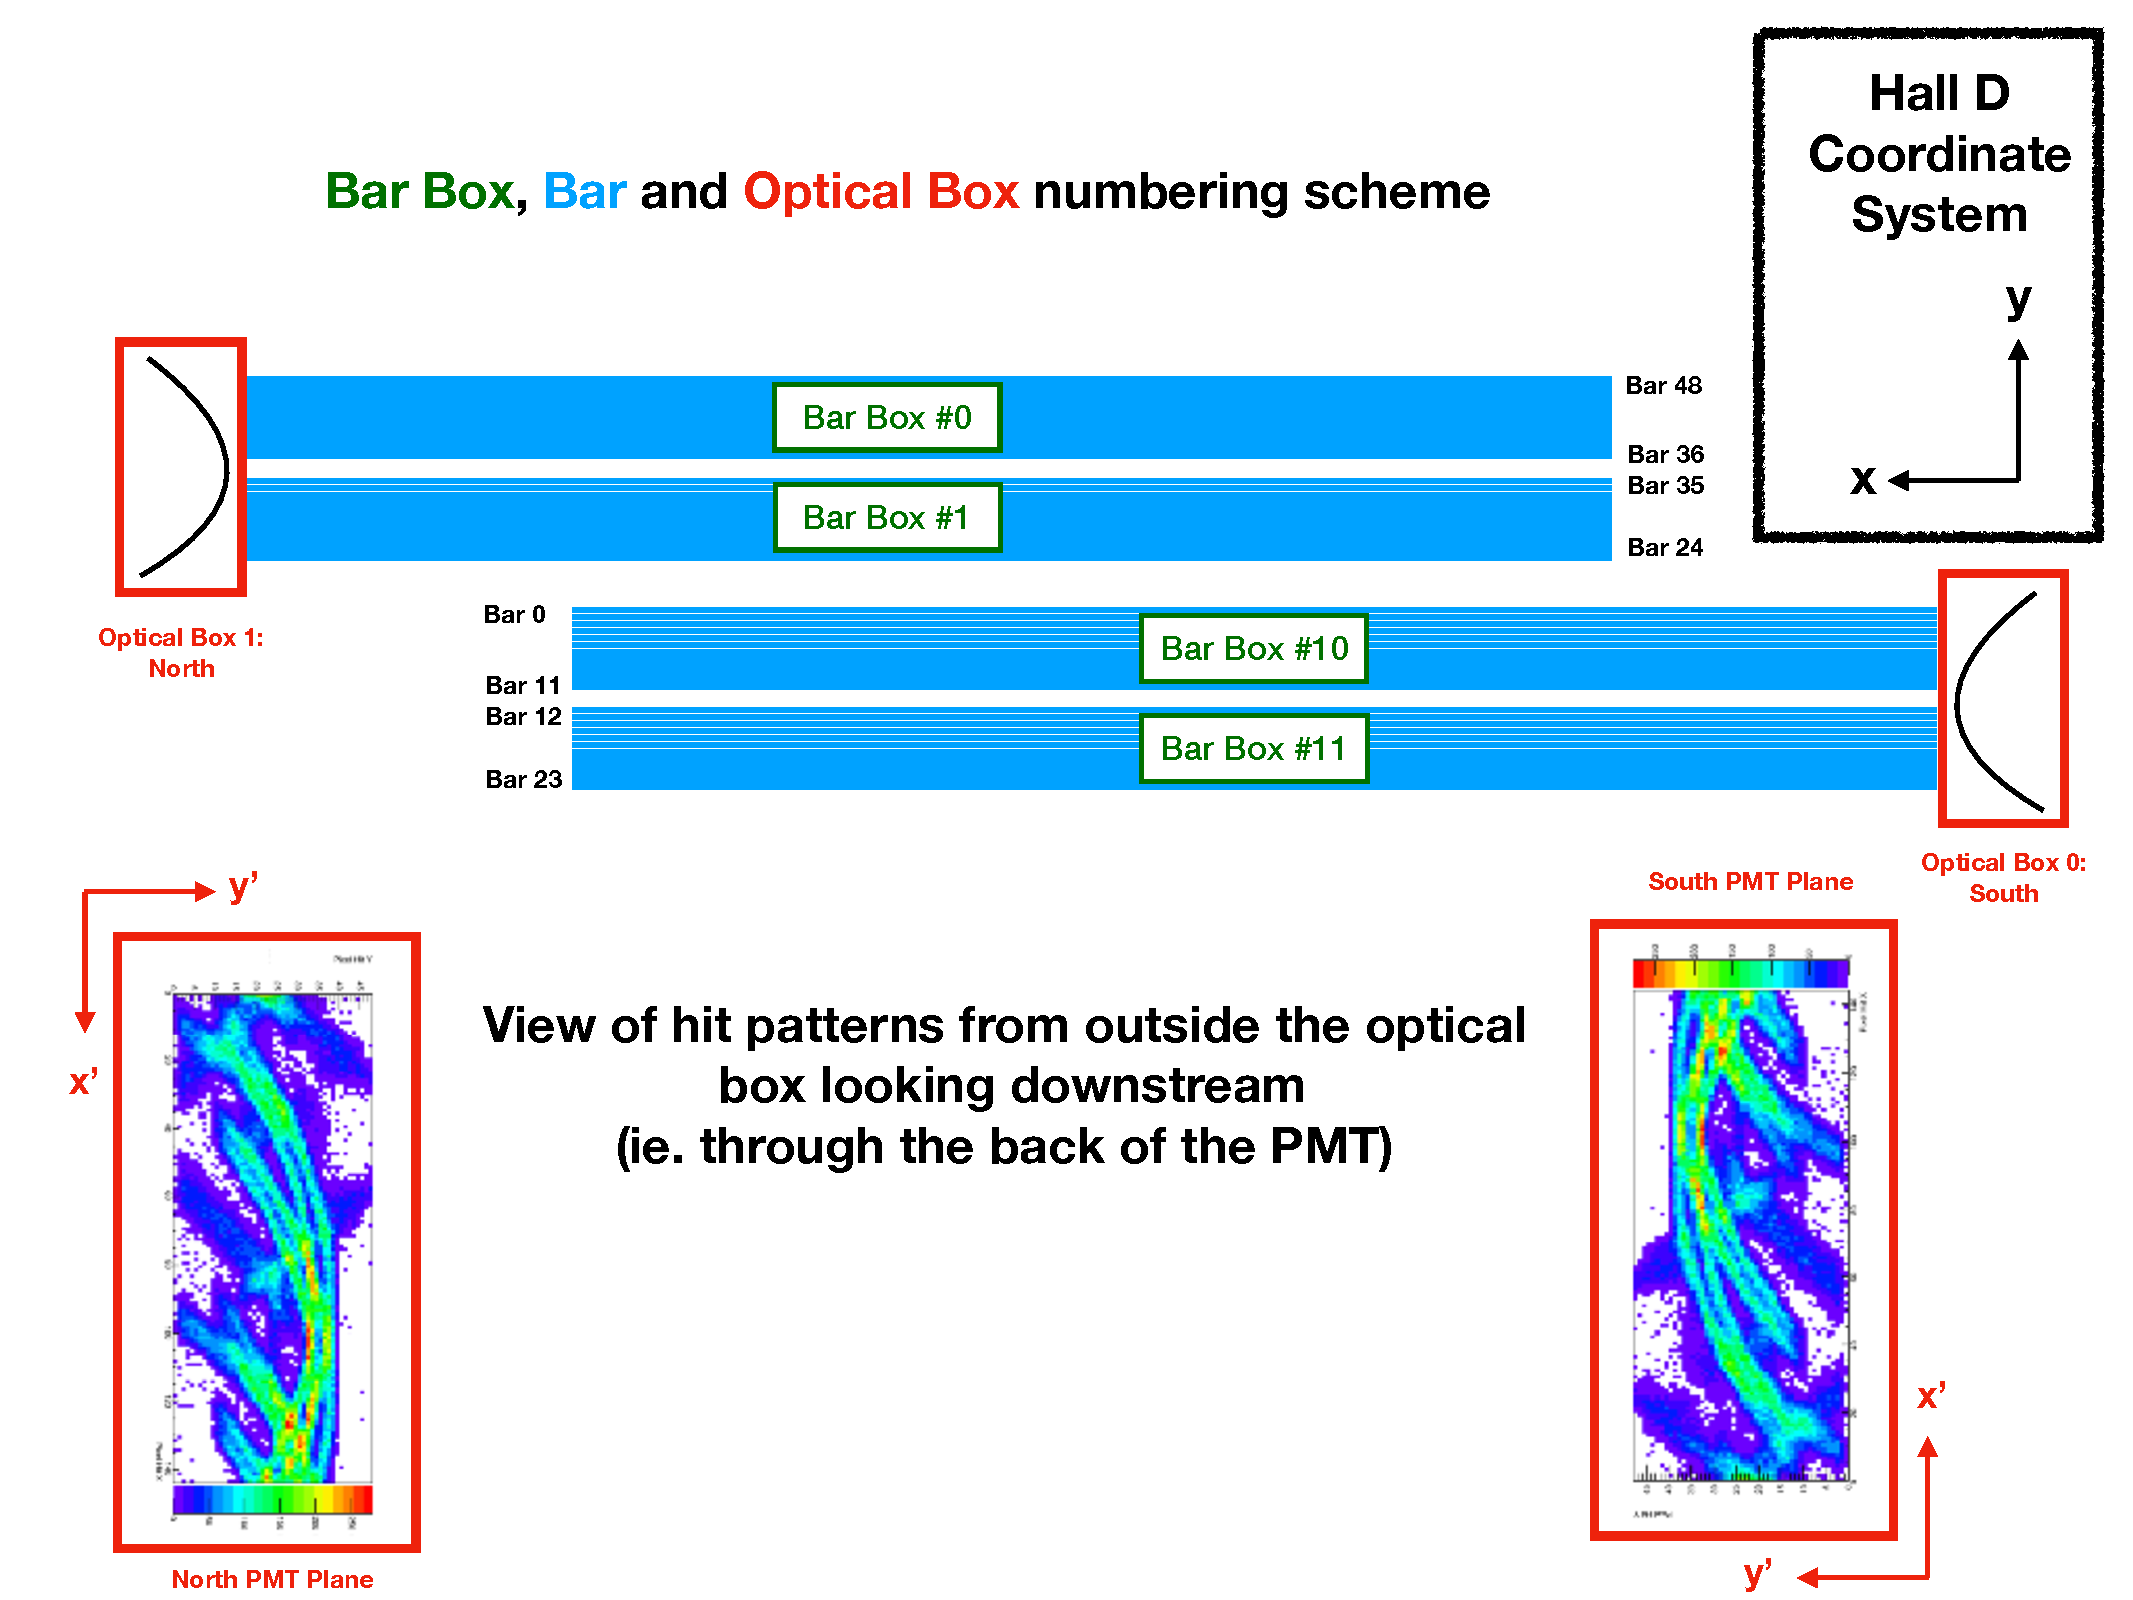
\includegraphics[width=0.98\textwidth]{pics/DIRC_Geometry11.pdf}\\
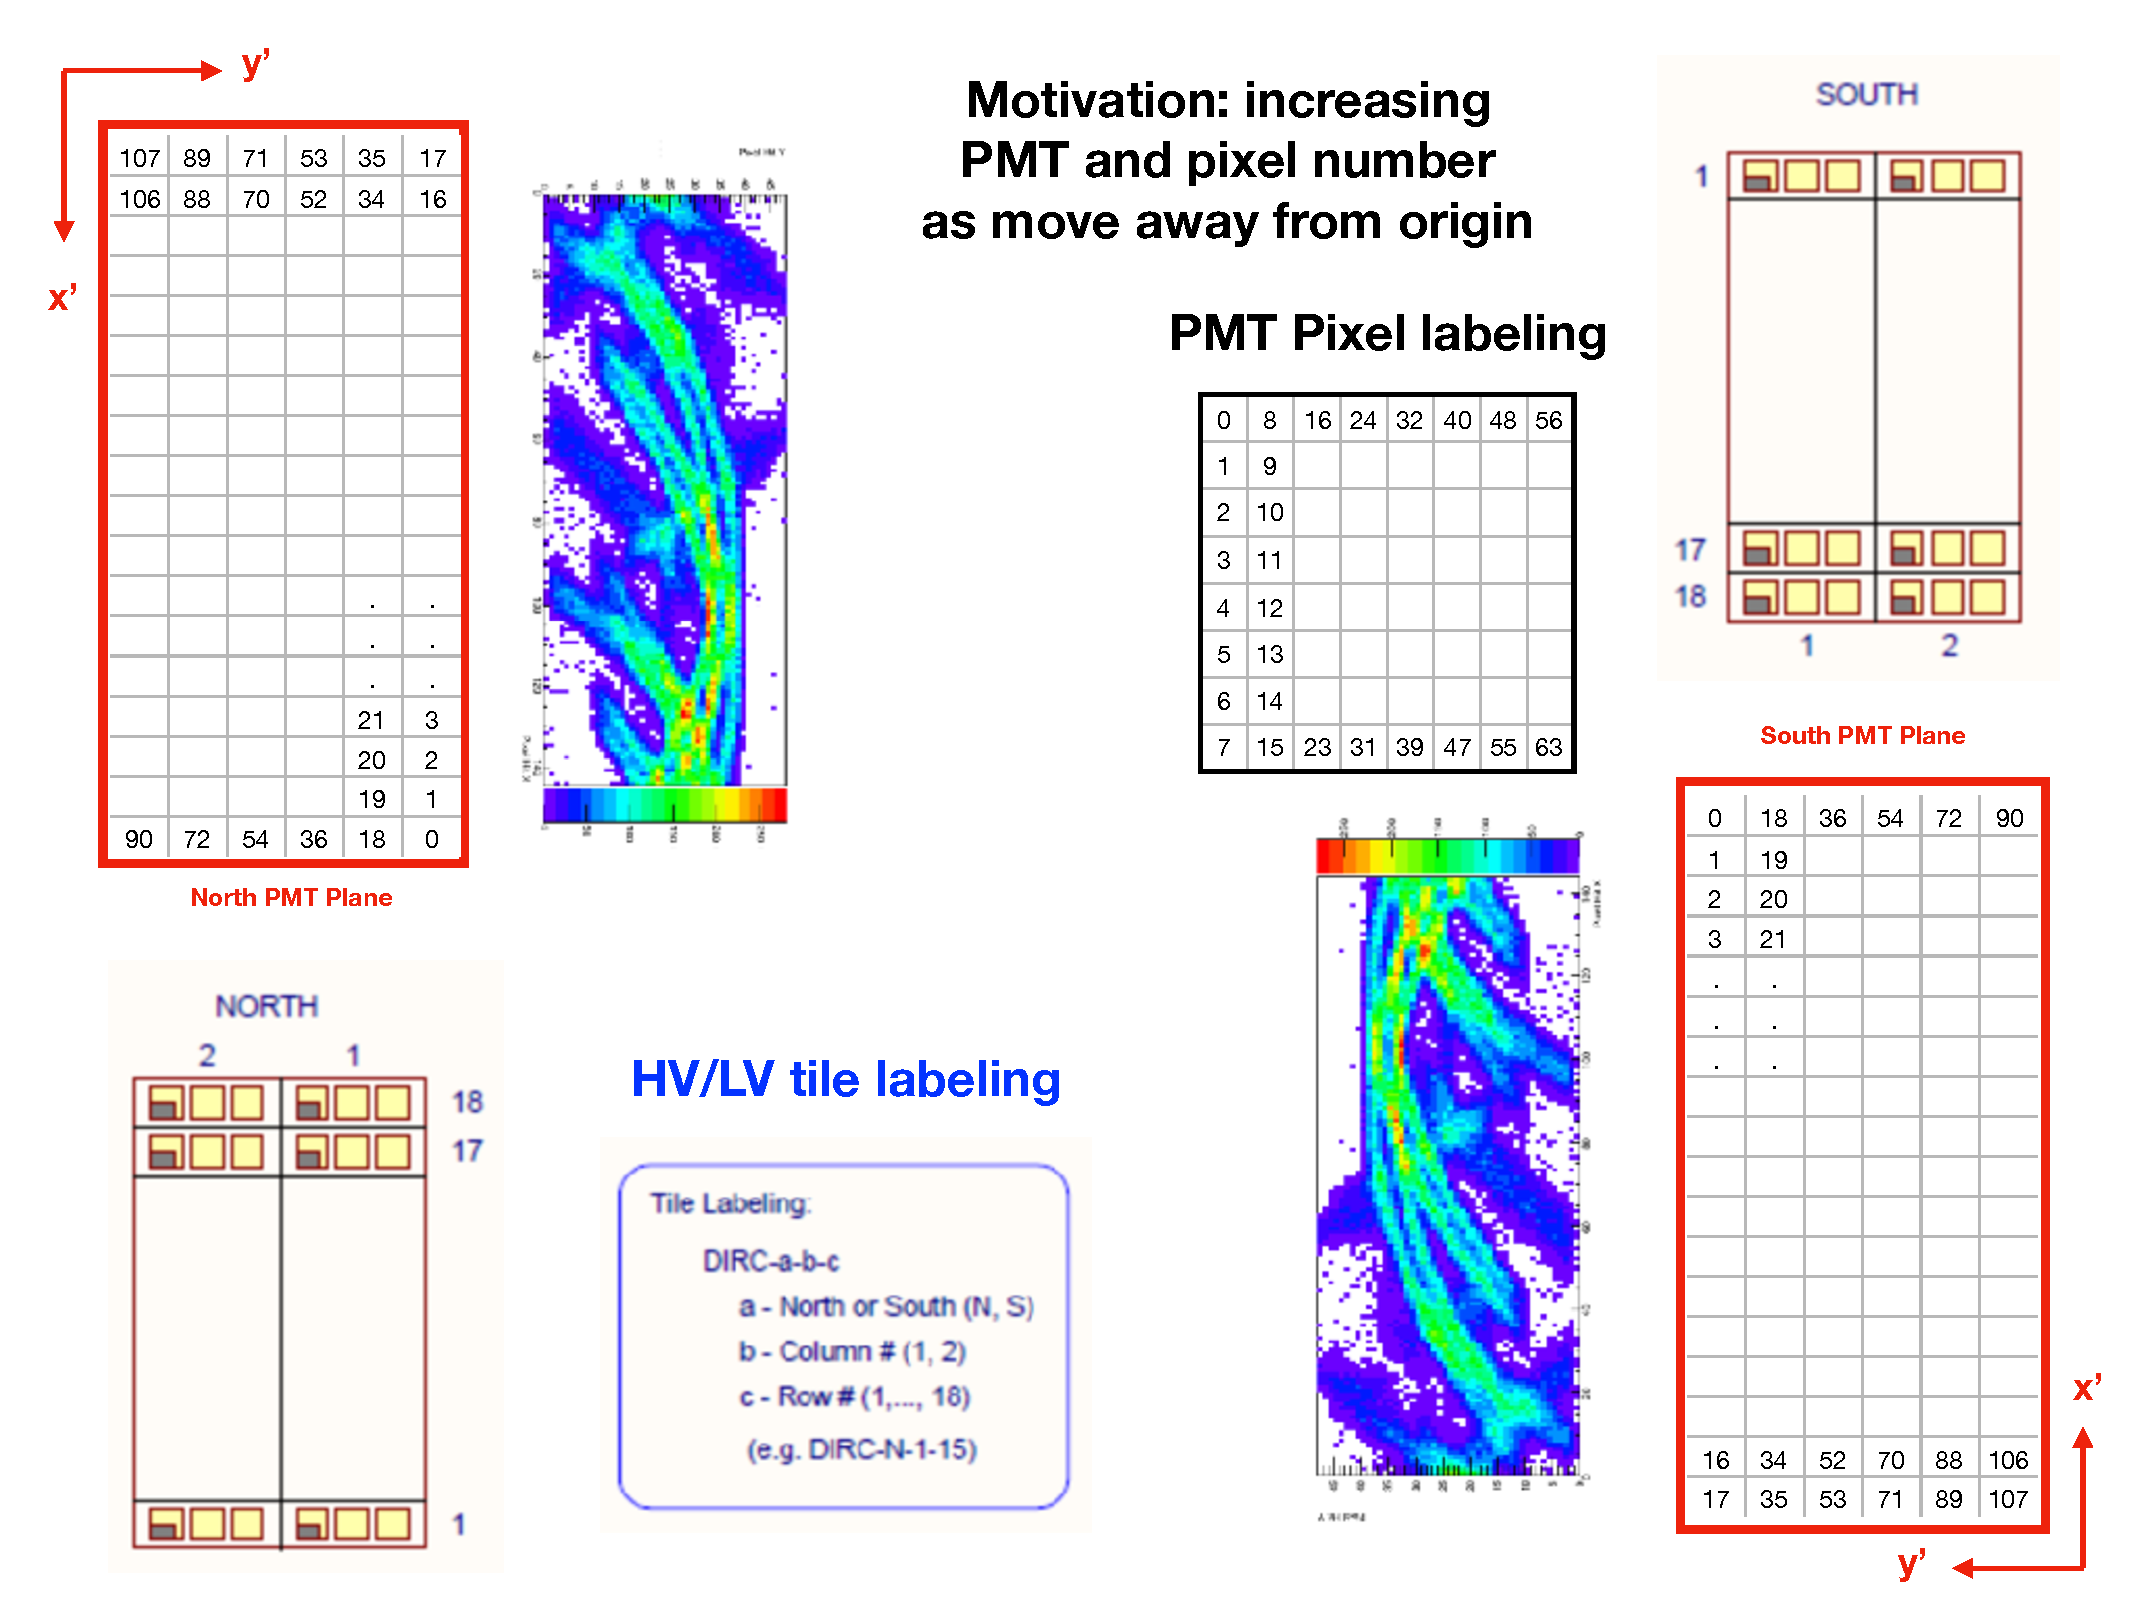
\includegraphics[width=0.98\textwidth]{pics/DIRC_Geometry22.pdf}
\caption{\label{pic:dirc2}
Numbering schemes of the DIRC constituents.
}
\end{figure}

The DIRC can be activated or deactivated by commenting in/out the corresponding line in the \texttt{main{\_}HDDS.xml} file (lines 82-83): 

\vspace{0.5cm}
\begin{center}
 \texttt{<!- - To simulate DIRC hits uncomment the line below - -> \\
    <!- -posXYZ volume="DIRC" X{\_}Y{\_}Z="0.0 0.0 595.0" /- ->} 
\end{center}
\label{eq:line}
\vspace{0.5cm}

The \texttt{DIRC} object, which is placed inside the virtual Hall D when the line above is active, is an auxiliary volume in a shape of a rectangular block containing all the DIRC consituents (see Fig.~\ref{pic:sim}). Its coordinates are defined in the global coordinate system of the hall, in which the $z$ axis goes along the beam, $x$ axis is parallel to the floor, and the $y$ axis is vertical. The target center is at $(0, 0, 65)$ cm. The center of the \texttt{DIRC} volume is at $z = 595$ cm.
Taking into account the z locations of the daughter volumes \texttt{DRCC} (composition holding the DIRC constituents), \texttt{DCML} (bar box), and \texttt{DCBR} (the radiator bar) the center of the radiator bar is currently at $z = 595 - 40 + 30 =585$ cm downstream the global 0. The distance from the center of the target ($(0, 0, 65)$ cm) is $585 - 65 = 520$ cm. The numbering schemes of individual volumes are represented in Fig.~\ref{pic:dirc2}.

\begin{figure}[!htb]
\centering
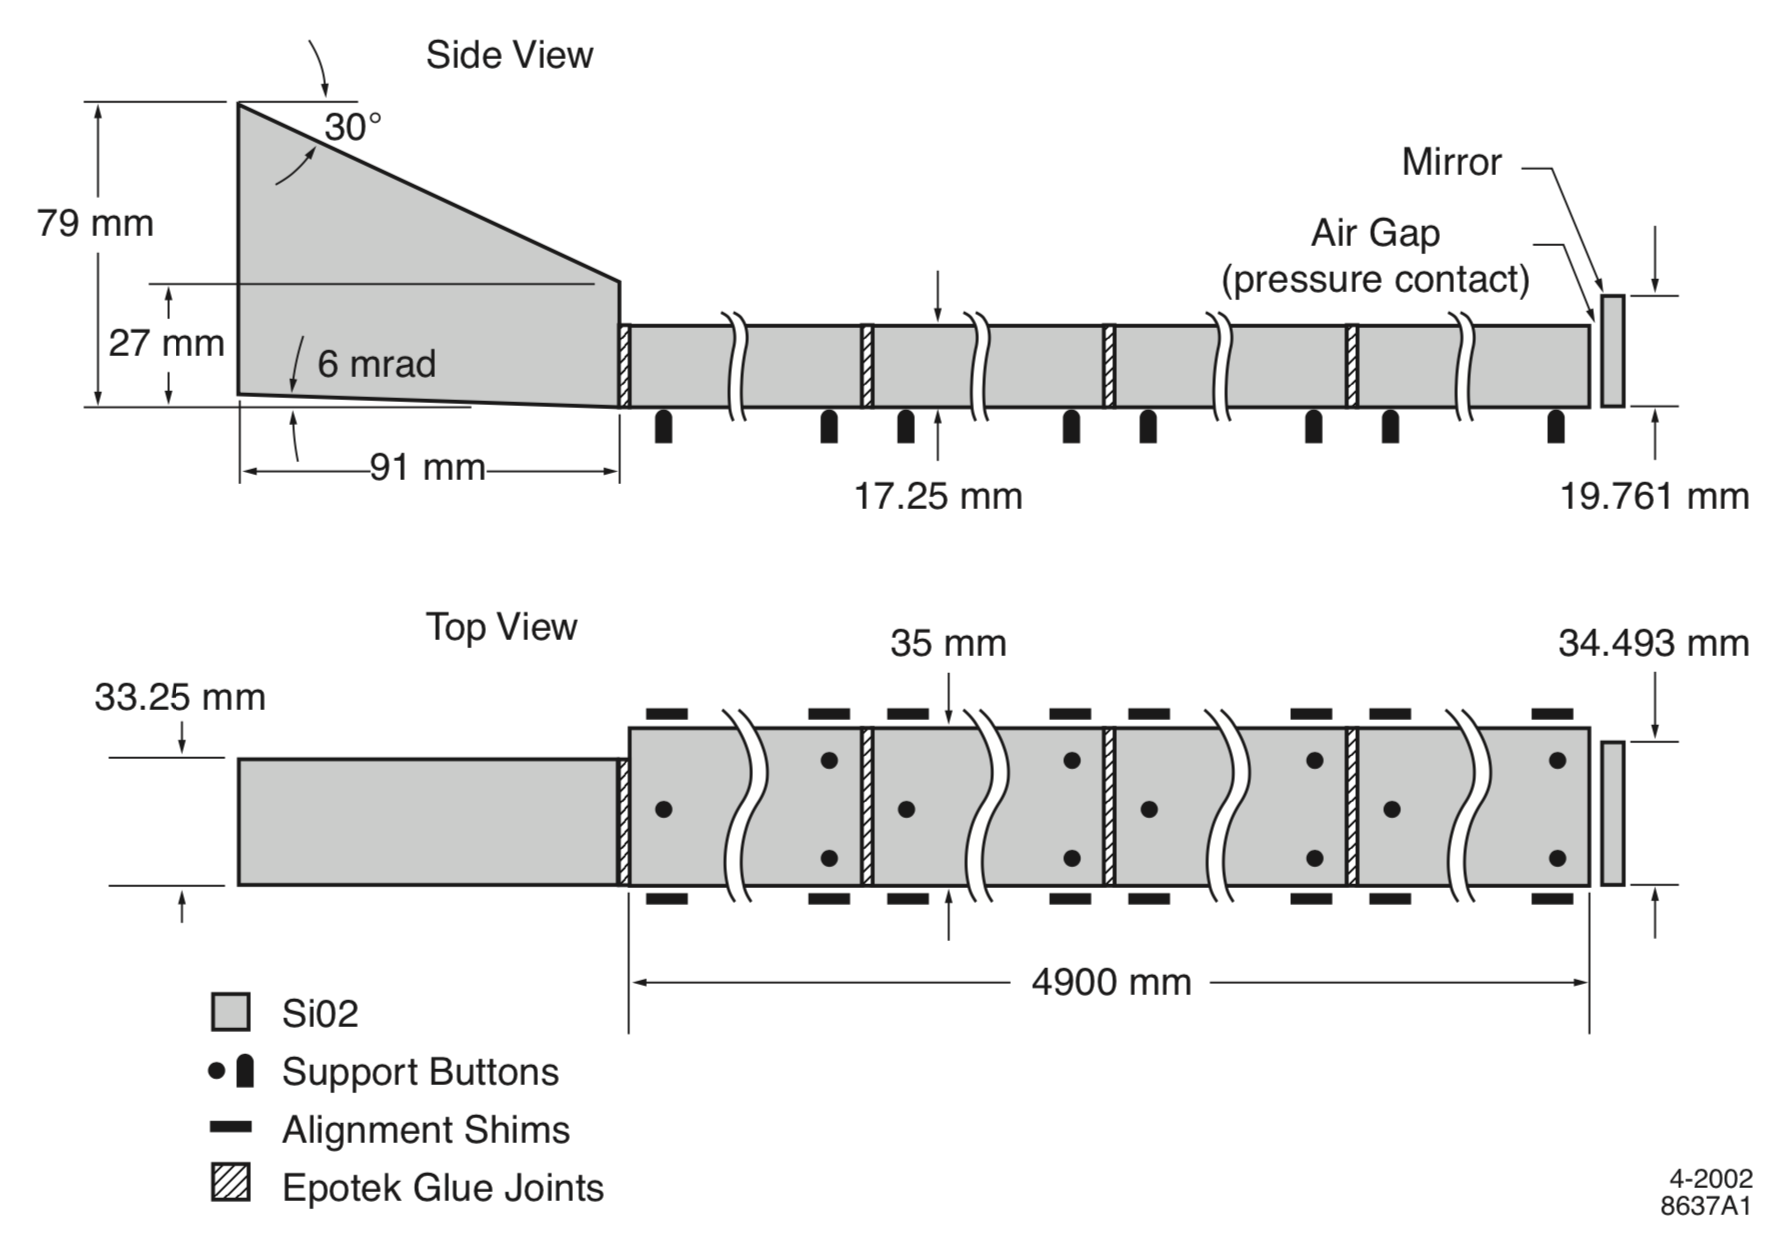
\includegraphics[width=0.8\textwidth]{pics/bars.png}
\caption{\label{pic:bar}
Schematic of the DIRC radiator bar in side and top view.
}
\end{figure} 

The structure of the radiator bar is shown in Fig.~\ref{pic:bar}. The mirror at the end of the bar has pressure contact with the fused silica bar, which implies an air gap. In simulation there is an air gap of $0.1$ mm between the mirror and the radiator bar. The schematic of the GlueX DIRC functional optical elements in the $yz$ projection, illustrating different materials used in the simulation, is shown in Fig.~\ref{pic:struct}.

\begin{figure}[!h]
\centering
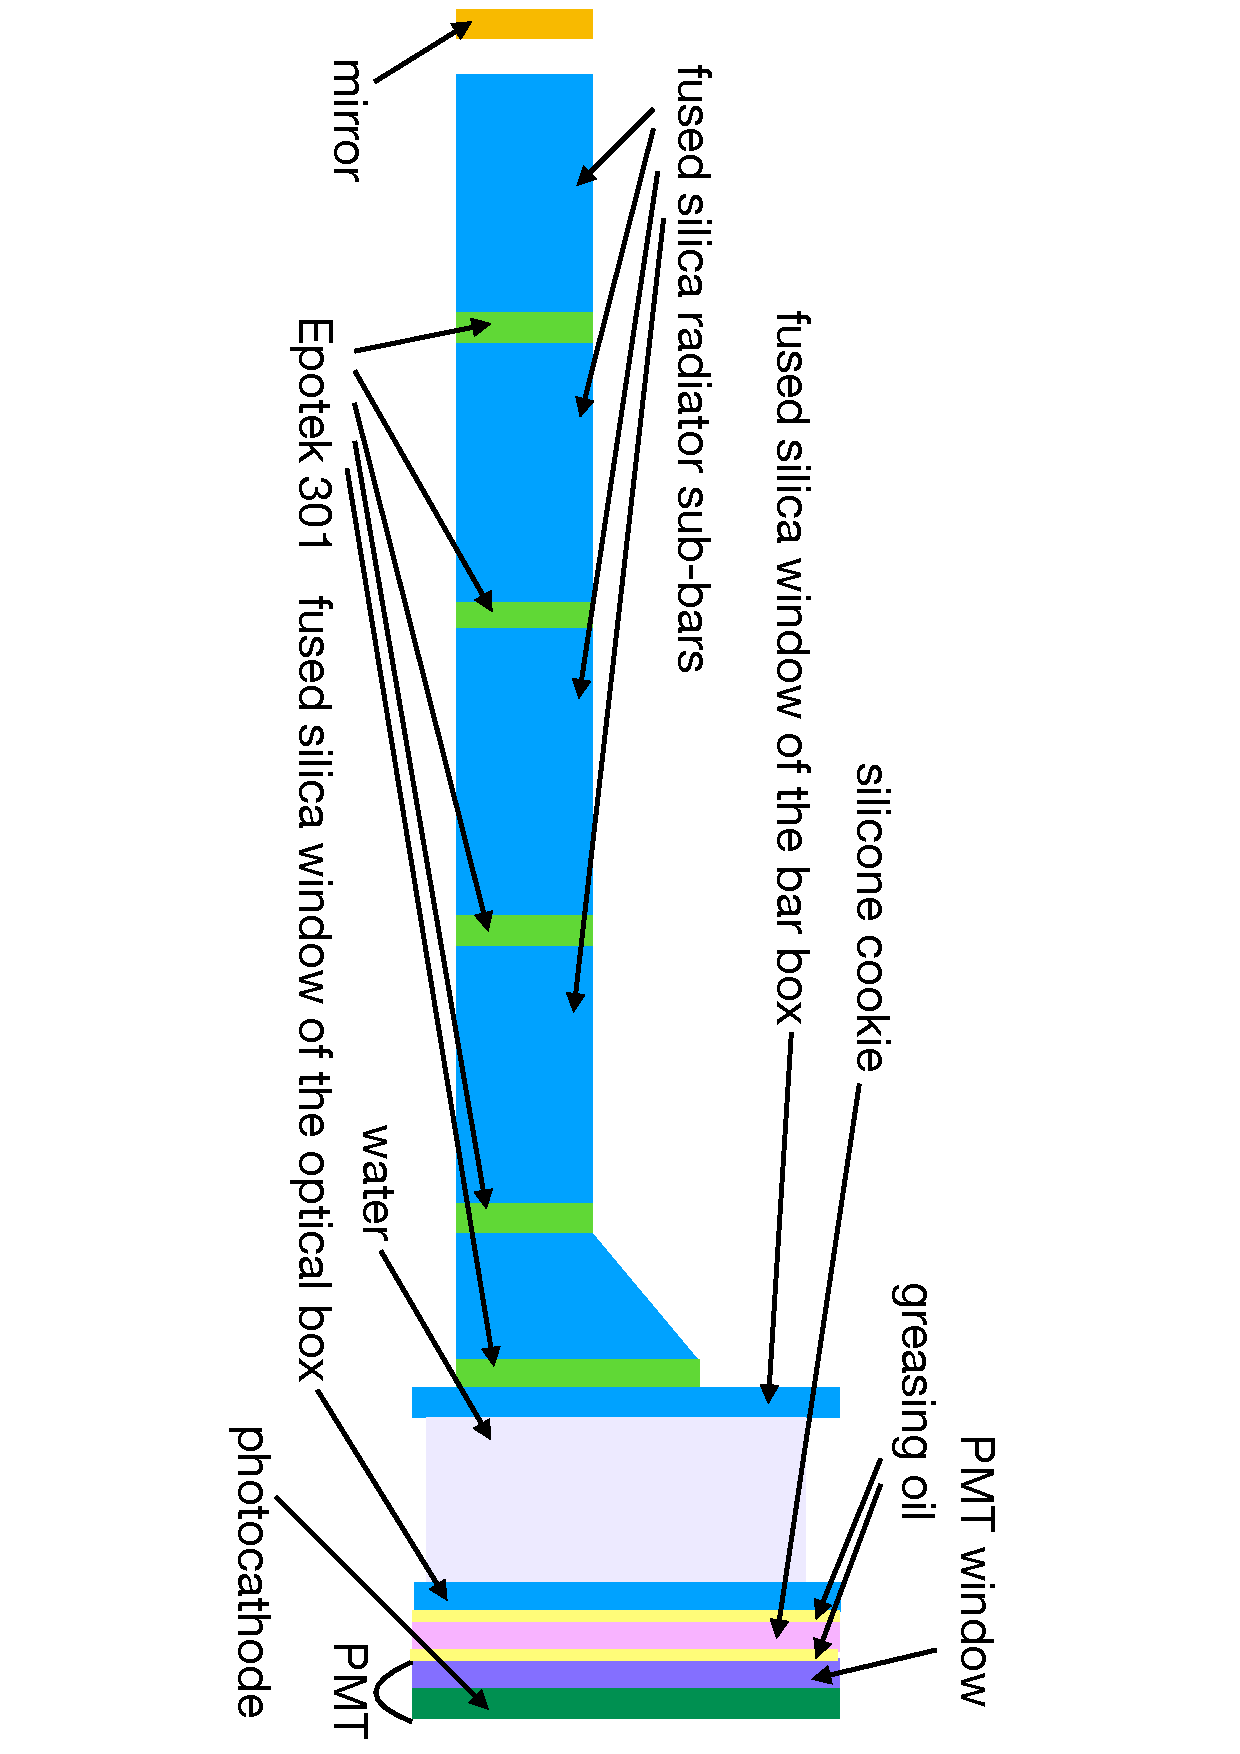
\includegraphics[angle=90,width=0.9\textwidth]{pics/struct1_crop.pdf}
\caption{\label{pic:struct}
Schematic of one bar box in projection along the radiator length showing all the materials used for the optical system. Mirrors inside the optical box are omitted. The components are shown not to scale.
}
\end{figure}

An array of MaPMTs is used to read out the signal. In the simulation, MaPMTs are implemented in a simplified way (see Fig.~\ref{pic:struct}) as a sequence of materials: a borosilicate window and a bialkali photocathode, which is sensitive. Sensitive here means, that when a photon enters this volume, a special function is called, which writes out the detector signal. The functionality of the sensitive elements of the GlueX DIRC is described in \texttt{GlueXSensitiveDetectorDIRC} class.


\subsection{Physical processes}

The general physical properties of the media (such as density, atomic weights, atomic numbers etc.) are used by Geant4 to simulate interactions of the particles with detector materials (e.g. Bremsstrahlung, ionization, production of secondary particles). If a material has, in addition, Cherenkov properties, then a particle can emit Cherenkov photons inside this material. The expectation value of the number of Cherenkov photons emitted per unit of trajectory $dN/dx$ is calculated according to the Frank-Tamm equation. During the propagation process of a charged particle inside the material with Cherenkov properties the number of photons produced within each step is generated according to a Poisson distribution with the mean of $\langle n \rangle = L_{step} \cdot dN/dx$. After the photons are produced they are propagated individually through the detector materials. The particles are transported inside the detector volume in an iterative process to discrete positions with a certain step size. At each of these positions a detector-specific routine is called by the Geant4 in order to process the simulated information inside its sensitive volumes. There, the current particle state (e.g. momentum, type, and mother-daughter relation) and the relevant processes during the current step (e.g. reflection, refraction) are available.

\begin{figure}[!h]
\centering
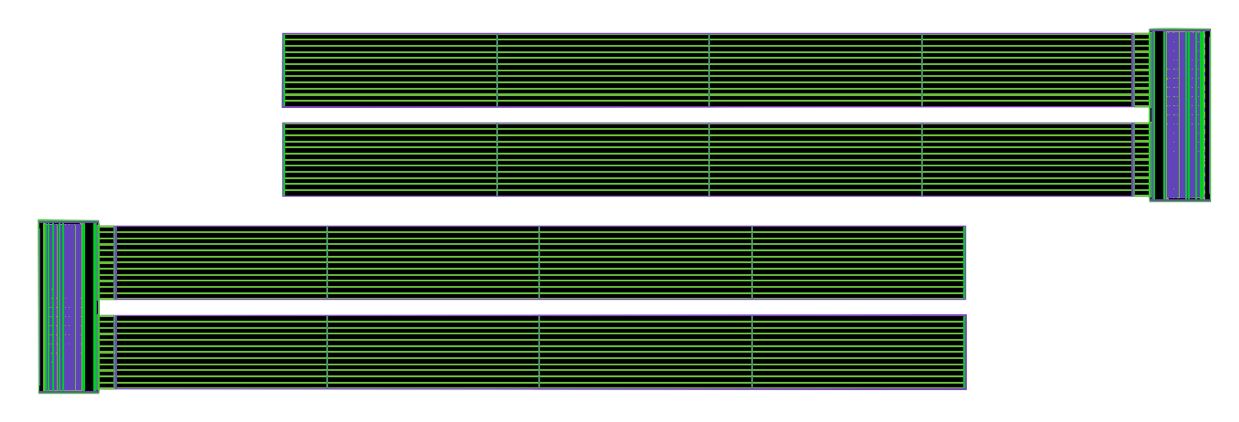
\includegraphics[width=0.8\textwidth]{pics/bars1.png}\\
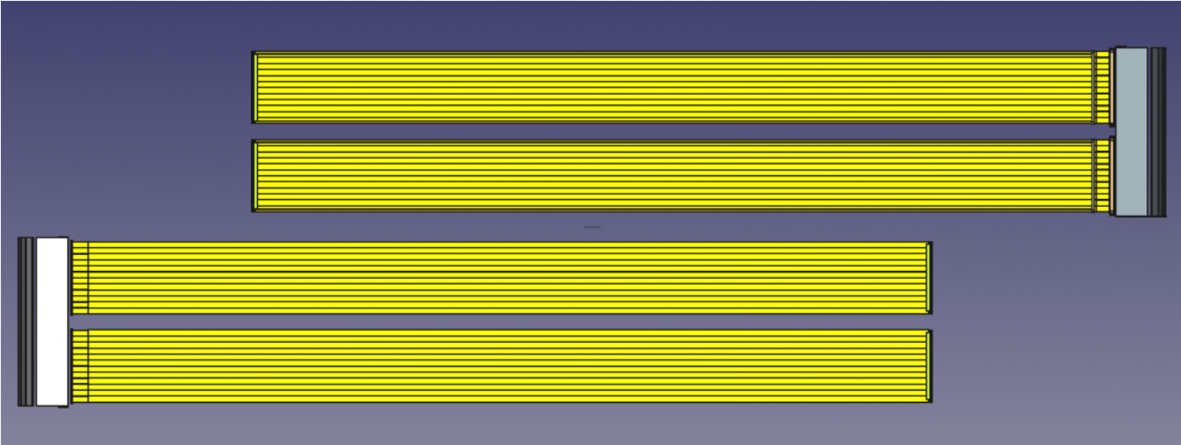
\includegraphics[width=0.8\textwidth]{pics/bars2.png}
\caption{\label{pic:dirc}
Simulation (top) and CAD drawings (bottom) of the GlueX DIRC.
}
\end{figure}  

\begin{figure}[!h]
\centering
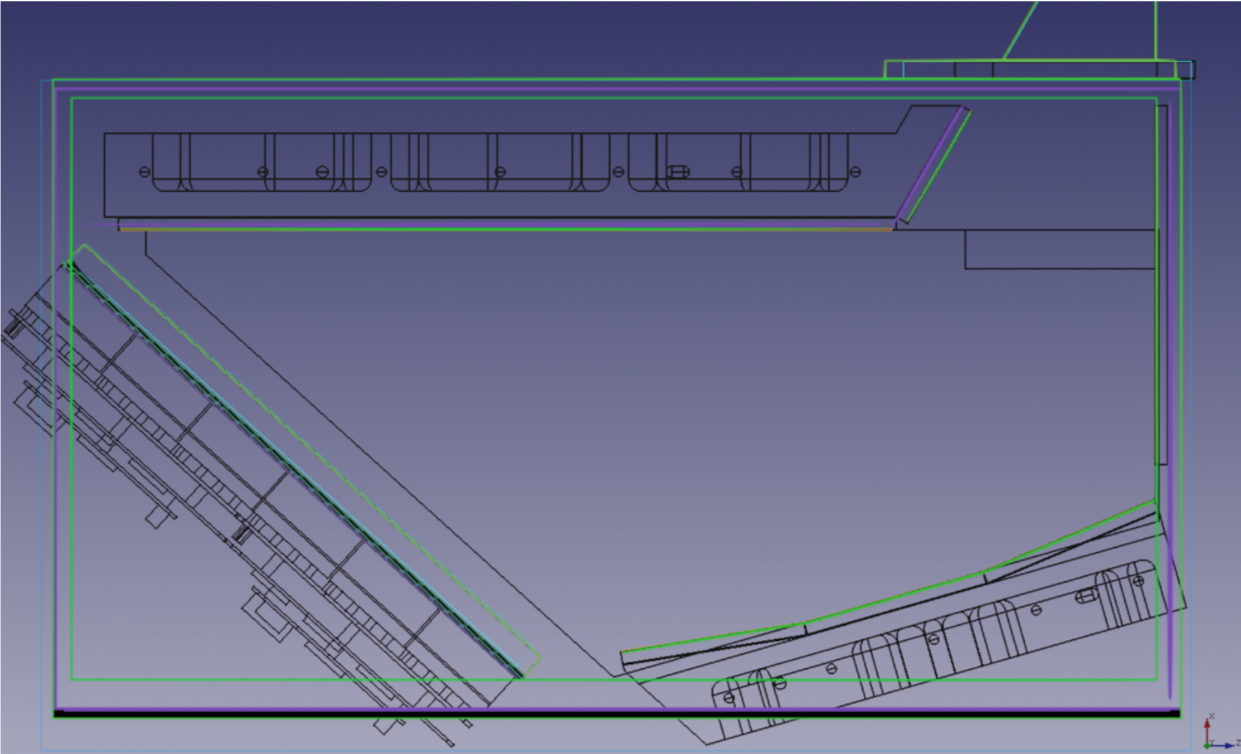
\includegraphics[width=0.8\textwidth]{pics/obgeom.png}
\caption{\label{pic:obg}
Geometry of the optical box overlayed with the CAD drawings illustrating the same locations of the mirrors. Green lines show optical elements in the simulation, black lines -- in the technical drawings.
}
\end{figure}

An important issue for the DIRC simulation is the realistic transport of Cherenkov photons through the optical elements of the detector from production to detection. Figures~\ref{pic:dirc} and~\ref{pic:obg} show that the current detector geometry matches the CAD technical drawings.

A high momentum charged particle produces at the order of $1000$ photons per cm of fused silica in the wavelength range $(300-700)$ nm. Only $30-60$ of them are expected to be detected. Typical Cherenkov photon energies are at the order of few eV. For proper estimation of the detector performance it is very important to predict realistic photon yields. Common reasons why a Cherenkov photon is not detected are the following:

\begin{itemize}
\item The material, where the Cherenkov photons is produced or currently propagating, might be non-transparen for the given wavelength -- the photon stops;
\item The photon does not satisfy the total internal reflection condition at the border between the radiator and the air around (and other interfaces) -- the photon leaves the radiator (or, more generally, the optical system of the detector) and is lost;
\item Some photons are reflected back on an interface between media with different refractive indices -- the photon is trapped inside some volume (or group of volumes);
\item The photon is absorbed in the material after it propagates a certain distance (the absorption properties of each material are defined by the absorption length as a function of the wavelength) -- the photon stops;
\item The photon is not detected because of the photon detection efficiency of the sensors (quantum efficiency for H12700 MaPMTs is shown in Fig.~\ref{pic:qe}) or the transport efficiency (described below)  -- the photon reaches the photosensor, but is not detected.
\end{itemize}

The physical processes in the materials are simulated by Geant4 based on the Cherenkov properties. The processes of total internal reflection, chromatic dispersion, transmission, and absorption of Cherenkov photons inside the optical elements of the GlueX DIRC are treated by Geant4, too.

A fraction of Cherenkov photons emitted by a charged particle, gets trapped inside the radiator due to the total internal reflection effect. They need to be transported from the origin to the readout end of the radiator bar. Cherenkov photons usually undergo at the order of several tens to several hundreds internal reflections inside a long BABAR DIRC bars on the way towards the readout end. The sides of the radiator in the reality are not perfect, and surface roughness causes a photon to get scattered in a random direction or escape from the radiator. In the simulation the radiator sides are perfectly polished leading to the fraction of transported photons to be $100\%$. In general, there are two ways to implement realistic transport efficiency into the simulation:

\begin{itemize}
\item The functionality of Geant4 (unlike Geant3) allows definition of an ``optical surface'' between two media with custom properties such as reflectivity and roughness. Then at each reflection off the radiator side, Geant4 decides according to the surface properties, to stop the photon or continue its transportation. It might be not straightforward to implement experimental results of the surface roughness measurements and make sure the simulation agrees with the measured data.
\item Transport efficiency can be calculated at the production stage for each photon based on the probability for a single reflection and the total number of reflections off the sides. This speeds up the simulation. Also, the measured surface roughness, which is usually based on the resulting decrease in the light intensity after $N$ reflections, is easy to implement.
\end{itemize}

We decided to follow the second method and apply the transport efficiency at the production stage as the following. The probability $P$ for a single reflection on the radiator side depends on the photon wavelength $\lambda$, incident angle of the photon $\alpha$, refractive index $n$, and the surface roughness $r$. According to scalar theory~\cite{scalar}:

\begin{equation}
P \approx  1 - \left( \frac{4\pi \cdot r \cdot \cos(\alpha) \cdot n(\lambda)}{\lambda} \right)^{2}, r \ll \lambda
\end{equation}

\begin{figure}[!h]
\centering
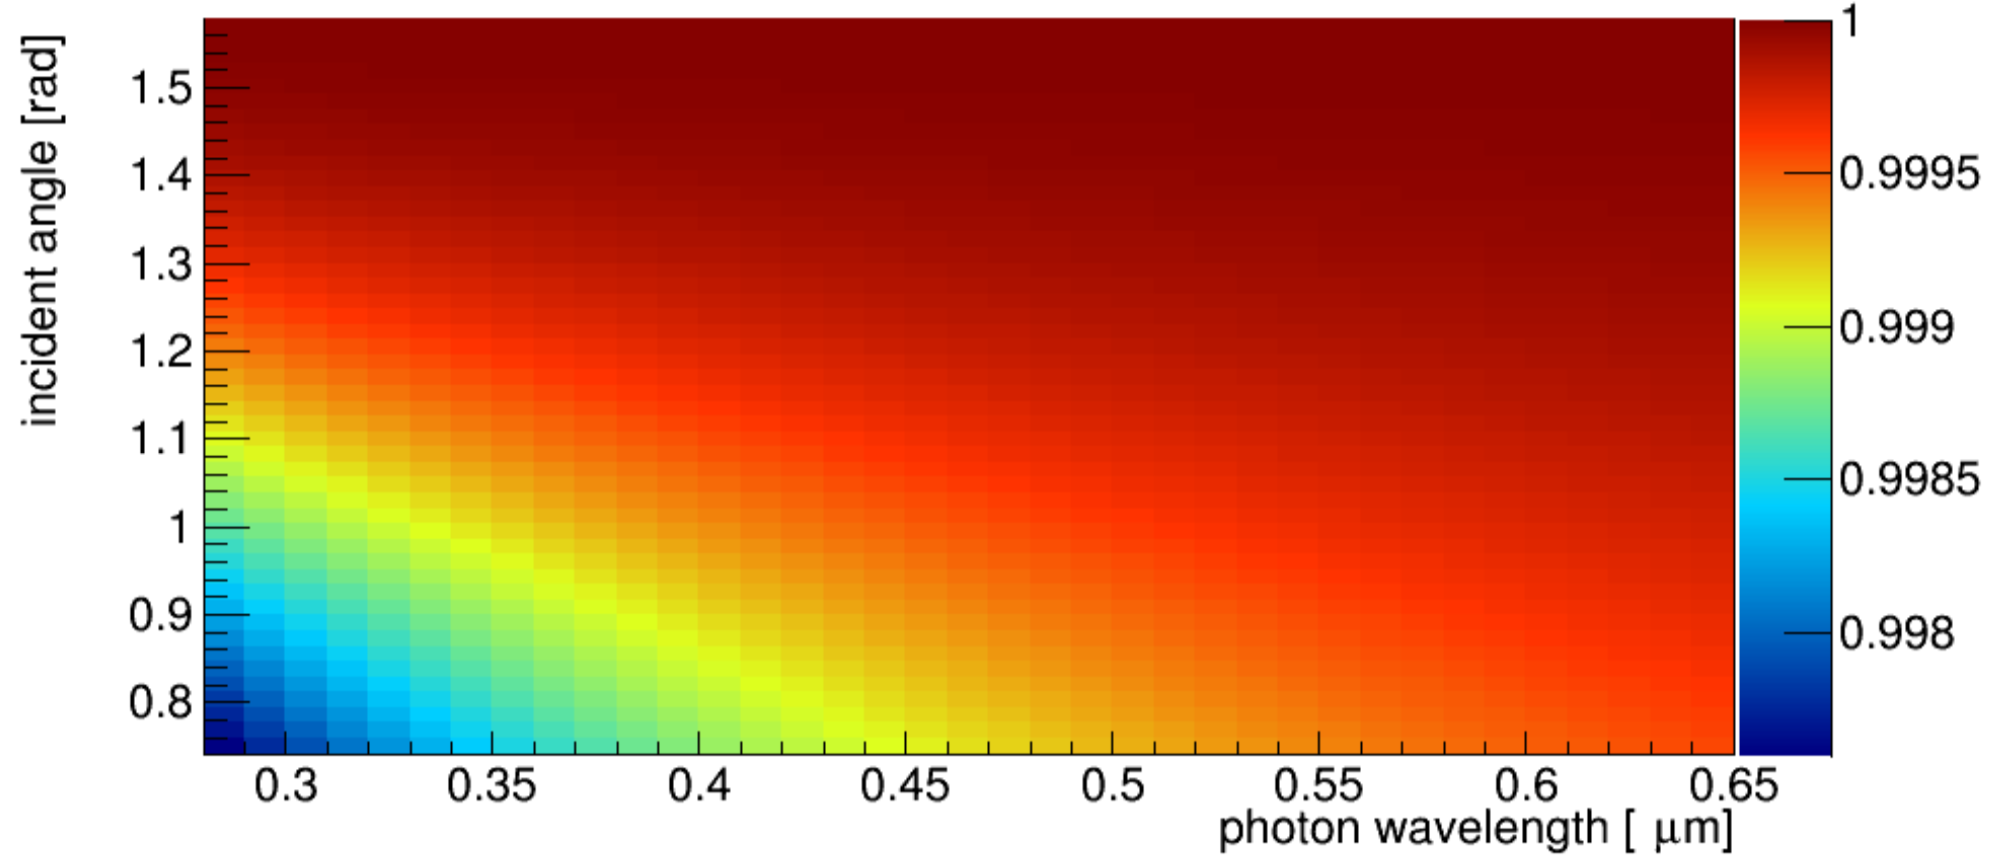
\includegraphics[width=0.8\textwidth]{pics/psurf.png}
\caption{\label{pic:sur}
Reflection coefficient $P$ as a function of the wavelength and incident angle of the Cherenkov photon.
}
\end{figure}

$P(\lambda,\alpha)$ is illustrated in Fig.~\ref{pic:sur}. The probability to survive the transpotation through the radiator can be calculated as $P_{total} = P^{N}$. Here $P_{total}$ is the transport efficiency for a given photon, and $N$ is the total number of reflections inside the radiator. We used experimental data of the transport efficiency, which agrees with the scalar theory for roughness value of $r \approx 5 A$~\cite{roughness}. Fig.~\ref{pic:tra} illustrates the impact of the transport efficiency on the photon yield for tracks hitting the bar (bar number 24 or 0 in Fig.~\ref{pic:dirc2}) closest to the beamline in different points along the $x$ axis. The effect is larger in the middle and decreases towards the ends of the bar. This correlates with the orientation of the Cherenkov cone inside the radiator: when a charged particle hits the middle of the bar, the Cherenkov cone is oriented perpendicularly to it, and photons have more reflections on the radiator sides than for the case, when the charged particle goes shallowly through the bar.

\begin{figure}[!h]
\centering
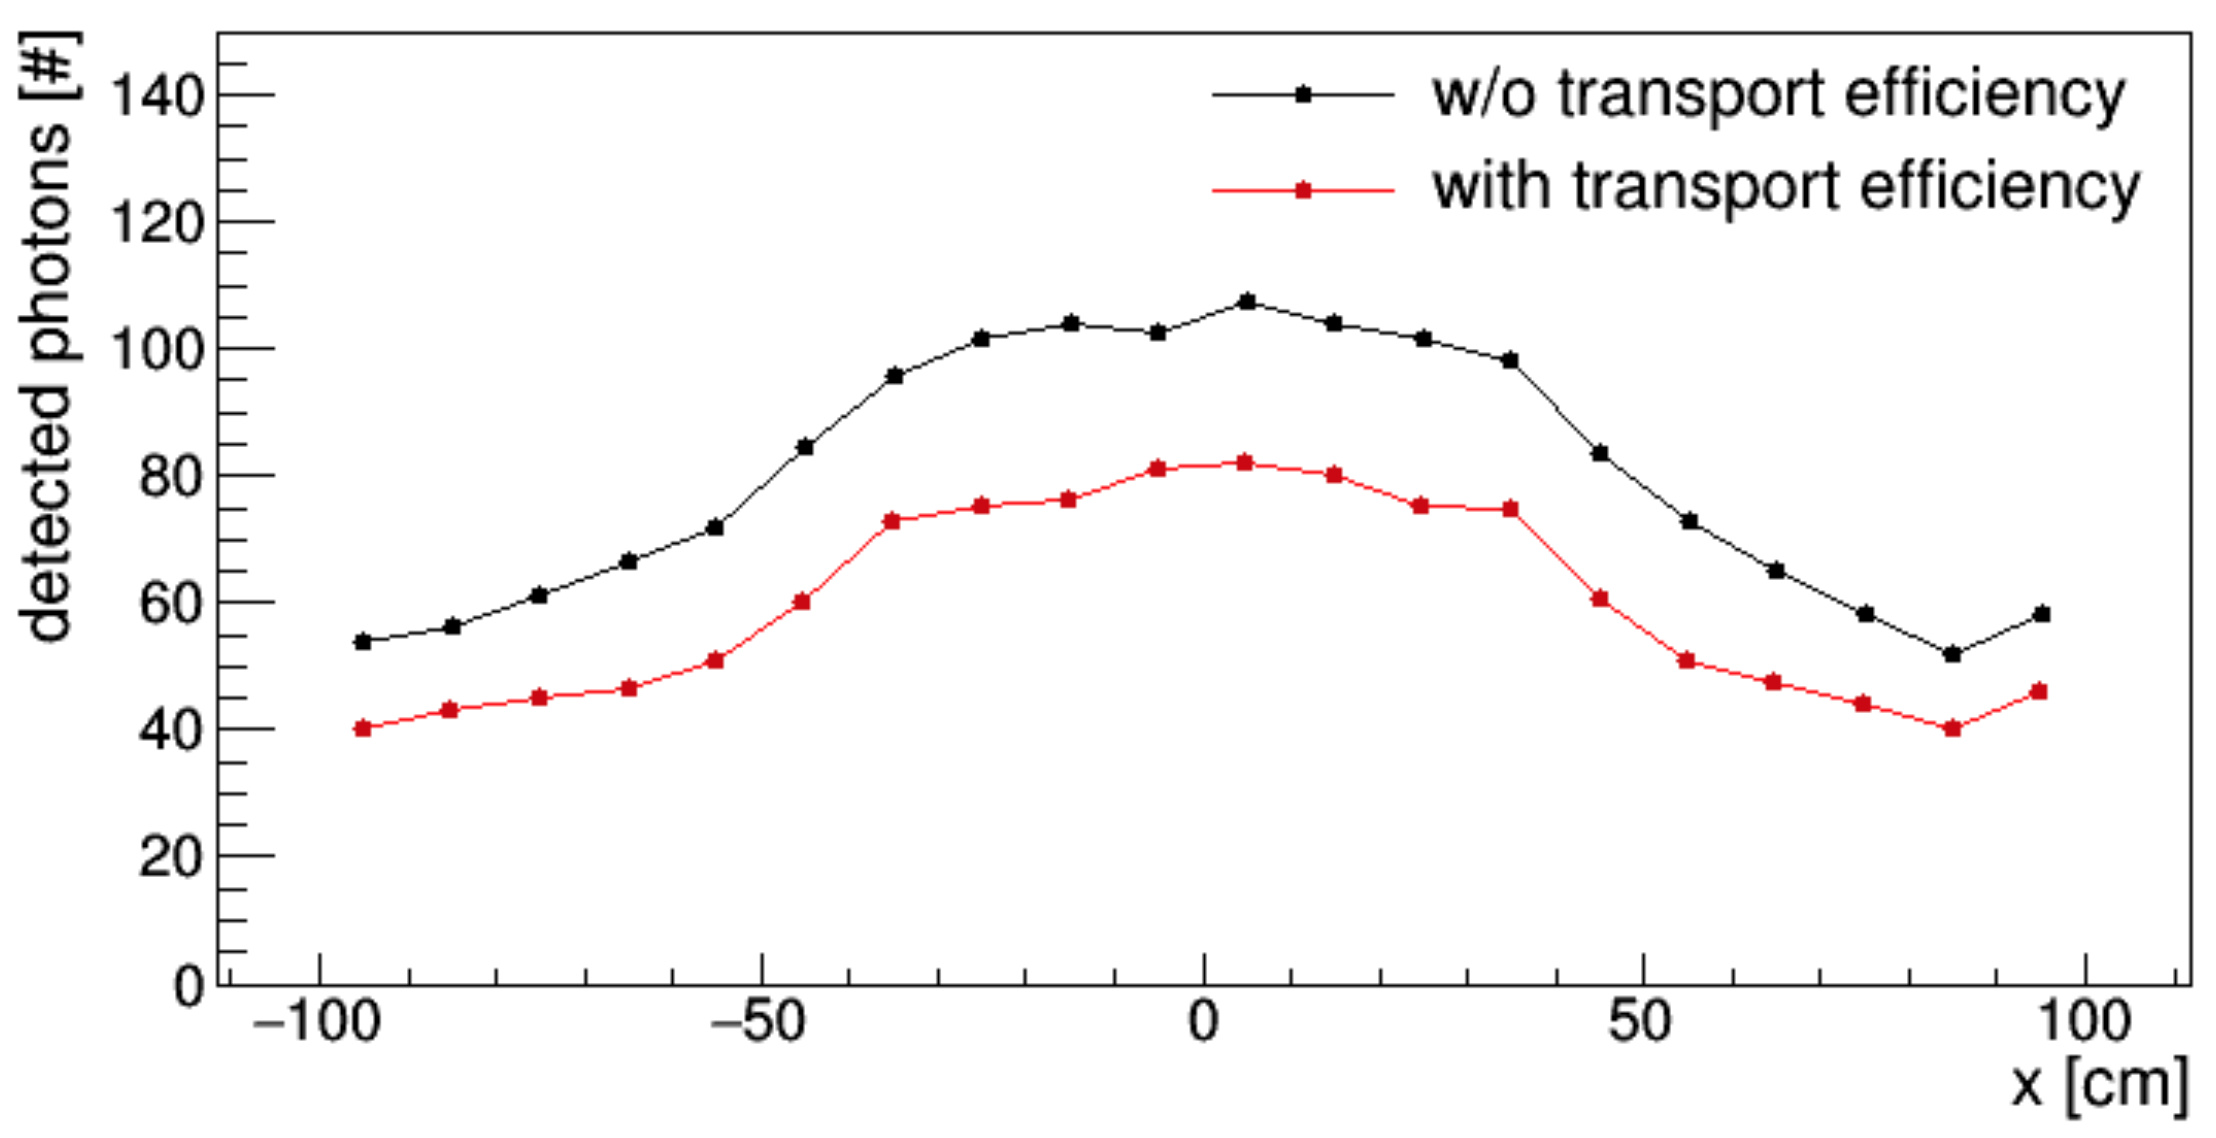
\includegraphics[width=0.8\textwidth]{pics/transport.png}
\caption{\label{pic:tra}
Impact of the transport efficiency on the photon yield. The study is based on $100k$ of $h'(2600)$ events. The photon yield is shown for the bar closest to the beamline (bar number 24 or 0 in Fig.~\ref{pic:dirc2}).
}
\end{figure}

The photon sensors are implemented in the simulation as a set of functional layers (see Fig.~\ref{pic:struct}). Propagation of Cherenkov photons through them is handled by Geant4. The detection efficiency, represented by the quantum efficiency of the photosensors (see Fig.~\ref{pic:qe}), is applied at the production stage to avoid tracing photons which are not going to be detected.

\begin{figure}[tb]
\centering
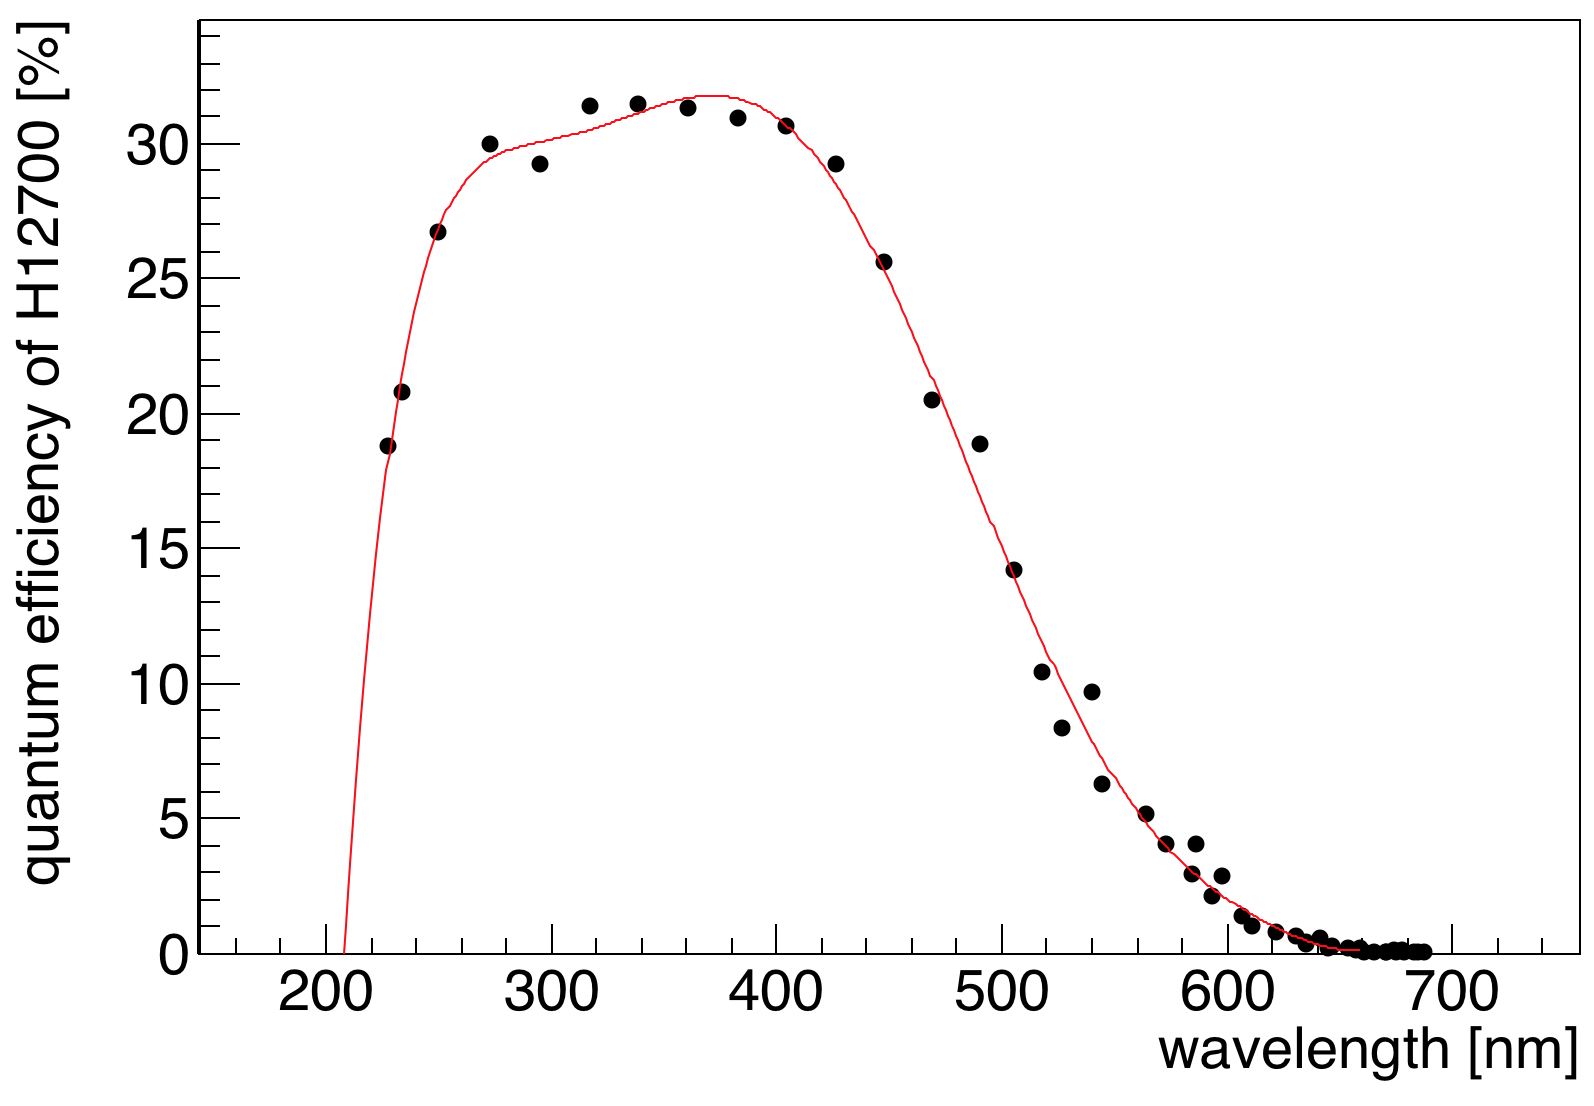
\includegraphics[width=0.5\textwidth]{pics/qe.png}
\caption{\label{pic:qe}
Quantum efficiency of photosensors Hamamatsu H12700. The red line shows a fit to the data points, extracted from the data sheet.
}
\end{figure}

The average bar dimensions are $35 \times 17.25 \times 4900 $ mm$^3$. The real measured bar sizes are being implemented into the geometry. 

The deterioration effects caused by imperfections of the physical shape of the radiators are not taken into account. The radiator bars in the detector simulation are perfect parallelepipeds, unlike in reality. Therefore, systematic smearing of the photon direction at every reflection inside the real radiator, which introduces an additional error to the reconstructed photon direction and therefore, to the obtained Cherenkov angle, is not (yet) taken into account.

\subsection{Material properties}

The nessesary Cherenkov properties of materials include refractive index and absorption lenght for a range of photon energies (see \texttt{hdds/Material{\_}HDDS.xml}).

The following table summarizes the sources for the material properties used in the simulation. The refractive index data was taken from (or compared to) (*) \\ \url{https://refractiveindex.info}. 

\vspace{0.5cm}
\begin{tabular}{| c | c | c |}
\hline
\textit{material} & \textit{refr. index} & \textit{abs. length} \\
\hline
Fused Silica & * and PANDA DIRC & same as for PANDA DIRC \\
\hline
Water & * & based on~\cite{water} and~\cite{water2} \\
\hline
Epotek 301 & same as for PANDA DIRC & same as for PANDA DIRC \\
\hline
cathode & $n = 2.7$ & $0.0001$ to stop photons \\
\hline
PMT window & * &  from Borosilicate Crown data sheet \\
\hline
RTV615 & $n = 1.406$ & our measurements \\
\hline
OCF 446 & $n = 1.46$ & copied from RTV615 \\
\hline
Optical air & $n = 1$ & did not double check \\
\hline
\end{tabular}
\vspace{0.5cm}


\subsubsection*{Epotek-301 optical glue}

The materials coupling together the elements of the detector optical system can introduce additional photon losses due to the poor Cherenkov properties. For the GlueX DIRC the sub bars are glued together with $d_{glue} = 50 \mu m$ thick layer of the optical glue Epotek $301$~\cite{Epotek}. The same glue was used to attach the small wedge and the bar box window. The refractive index and absorption length for Epotek-301 were taken from the PANDA Barrel DIRC simulation (PandaRoot).

\subsubsection*{Borosilicate glass}

H12700 PMTs can have either borosilicate glass or UV glass. GlueX DIRC has H12700 with borosilicate glass. The thickness of the PMT window is $1.5$ (see specs sheet). The absorption length from the Schott Borofloat 33 data sheet is shown in Fig.~\ref{pic:gla}. The transmittance values should be corrected for Fresnel reflection. Fresnel reflection of the air-glass interface can be calculated as:

\begin{equation}
R = \Bigl( \frac{n_1 - n_2}{n_1 + n_2} \Bigr)^{2} = \Bigl( \frac{1.53 - 1}{1.53 + 1} \Bigr) ^{2} \approx 4.4\%,
\label{eq:fre}
\end{equation}

\noindent where $n_1 = 1.53$ -- refractive index for borosilicate glass, $n_2 = 1$ -- refractive index for air. The light passed the following tnerfaces: air-glass, glass-air. On each of two interfaces the Fresnel reflection should be taken into account leading to $R_{total} = 8.6\%$. The incident light was partly reflected ($R_{total}$), partly absorbed ($A$), and partly transmitted ($T$): $ R_{total} + T + A = 1$. For the absorption length $\lambda$ we need $1 - A = R_{total} + T = e^{-x/\lambda}$. 

\begin{figure}[htb]
\centering
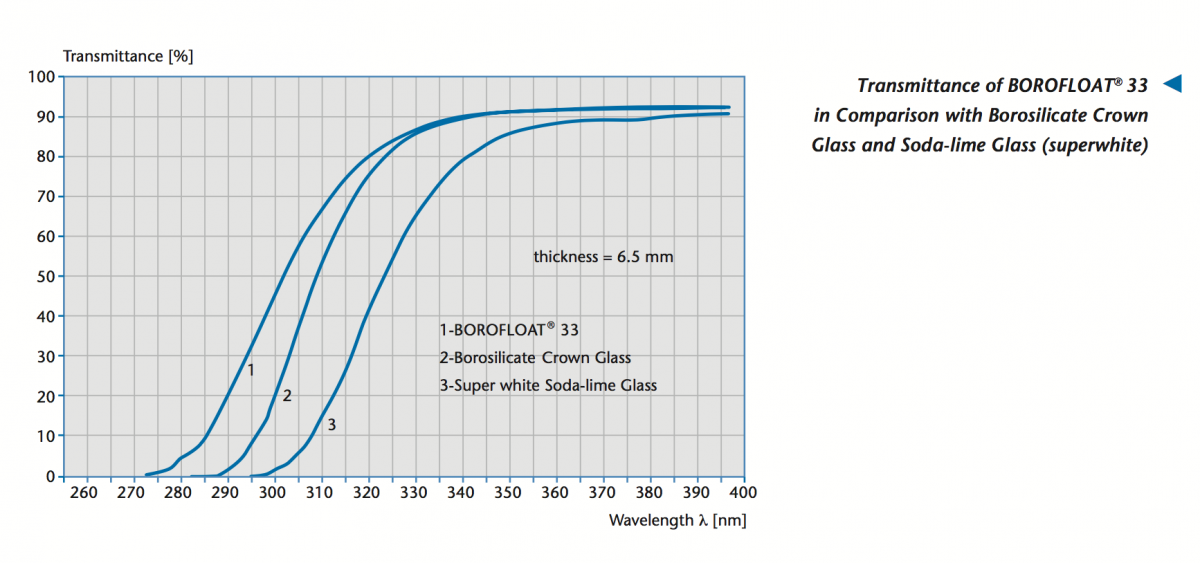
\includegraphics[angle=0,width=0.8\textwidth]{pics/glass.png}
\caption{\label{pic:gla}
Transmittance for the borosilicate glass.
}
\end{figure}

\begin{equation}
\lambda = -x/\log(R_{total}+T) = -0.15/\log(0.086+T),
\label{eq:lam}
\end{equation}

\noindent here we assume glass thickness $x = 0.15$ cm. The following table shows absorption length for the borosilicate glass extracted from the Fig.~\ref{pic:gla} plot (line 2):

\begin{center}
\begin{tabular}{| c | c | c | c | c | c | c | c |}
\hline
wavelength [nm] & 280 & 300 & 310 & 320 & 340 & 380 \\
\hline
transmittance & 0 & 0.20 & 0.55 & 0.75 & 0.90 & 0.92 \\
\hline
$\lambda$ [cm] & 0 & 0.12 & 0.33 & 0.84 & 10.6 & 25.0 \\
\hline
\end{tabular}
\end{center}

\subsubsection*{Silicone cookies}

The material used to produce cookies is RTV615 by Momentive. The mixing ratio is $100 : 2.5$ (unlike the default mixing ratio of $10 : 1$), which makes the pad softer. The thickness of the real cookies is $\approx 0.17$ cm, and the area is $5.2$ cm times $15.8$ cm. For the simulation the refractive index of the cookies is set constant $n = 1.406$, and the absorption length is taken from our measurements (see Fig.~\ref{pic:coo}). All the custom-made cookies have similar and good transmittance properties independently on the curing method or mixing ratio.

\begin{figure}[!tb]
\centering
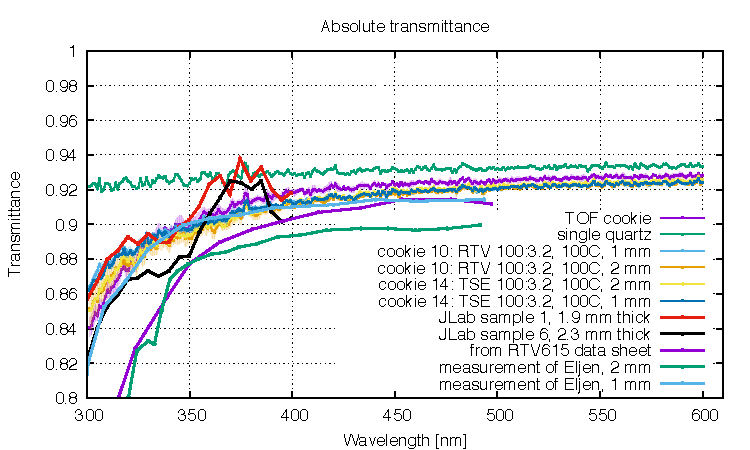
\includegraphics[angle=0,width=0.9\textwidth]{pics/transmittance1.pdf} \\
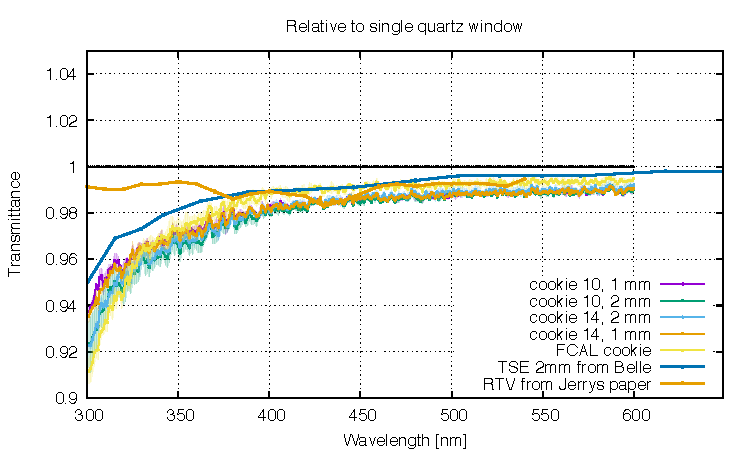
\includegraphics[angle=0,width=0.9\textwidth]{pics/cookie10_relQuartz.pdf}
\caption{\label{pic:coo}
Transmittance measurements for a set of custom-made silicone cookies. Absolute values (above), and relative to a single quartz window  (below). FCAL cookie is a pre-made cookie by Momentive (same RTV615 material, thickness $2$ mm). The data for TSE 2 mm cookie is taken from a plot on Belle II TOP cookies transmittance, which had poor resolution. The paper mentioned here is SLAC-PUB15942.
}
\end{figure}

The absorption length of the silicone was extracted from the absolute transmittance measurements (see Fig.~\ref{pic:coo} above). Transmittance was measured for the cookie sandwiched between two fused silica windows. Fresnel reflection of the air-fused silica interface can be calculated similarly to~(\ref{eq:fre}) using $n_1 = 1.47$ -- refractive index for fused silica leading to $R = 3.6 \%$. The total reflection loss for a single quartz window in air is then $R_{total} = 7.1 \%$. This estimation agrees with the absolute transmittance of quartz shown in Fig.~\ref{pic:coo} above (we can neglect the absorption inside the FS window). The absorption length for the silicone cookie can be calculated using~(\ref{eq:lam}), and we neglect the Fresnel reflections on the FS-cookie interface, which is about $R = 0.05 \%$.

%To extract absorption length for the silicone cookie, we have to account for the Fresnel reflections of the measured sample. Fresnel reflections on the FS-cookie interface is about $R = 0.05 \%$, so we neglect it. The incident light was partly reflected ($R$), partly absorbed ($A$), and partly transmitted ($T$): $ R_{total} + T + A = 1$. For the absorption lenght $\lambda$ we need $1-A = R_{total}+T = e^{-x/\lambda}$. 

%\begin{equation}
%\lambda = -x/\log(R_{total}+T) = -0.2/\log(0.071+T),
%\end{equation}

%\noindent here we assume cookie thickness of 2 mm. 
The following table shows absorption length for the silicone extracted from the Fig.~\ref{pic:coo} plot:


\begin{center}
\begin{tabular}{| c | c | c | c | c | c|}
\hline
wavelength [nm] & 300 & 350 & 400 & 450 & 600 \\
\hline
transmittance & 0.85 & 0.89 & 0.91 & 0.915 & 0.915 \\
\hline
$\lambda$ [cm] & 2.43 & 5.03 & 10.43 & 14.2 & 14.2 \\
\hline
\end{tabular}
\end{center}

\subsubsection*{Greasing silicone fluid OCF-446}

The Nye Lubricants OCF-446 silicone fluid is used to grease the cookies and therefore create a good optical coupling. The usage of particularly this product was inspired by the Belle II TOP experience. To create this material, we need to put molecular structure of it. OCF-446 is a vinyl terminated (diphenylsiloxane) dimethylsiloxane copolymer commonly referred to as a Phenyl Silicone. The molecular structure of this material is shown in Fig.~\ref{pic:ocf}. The diphenylsiloxane group is repeated $m$ times in this schematic, and dimethylsiloxane group -- $n$ times. For the simulation I need the number of atoms of each type in one molecule. I assume that $m = n = 1$, which leads to $20$ $C$ atoms, $30$ $H$ atoms, $4$ $Si$ atoms, and $3$ $O$ atoms. The data on the refractive index of OCF-446 is poor: there is only one measurement $n = 1.46$ at $\lambda = 589.3$ nm, which corresponds to photon energy of $\approx 2$  eV. No data on absorption length is available.

\begin{figure}[htb]
\centering
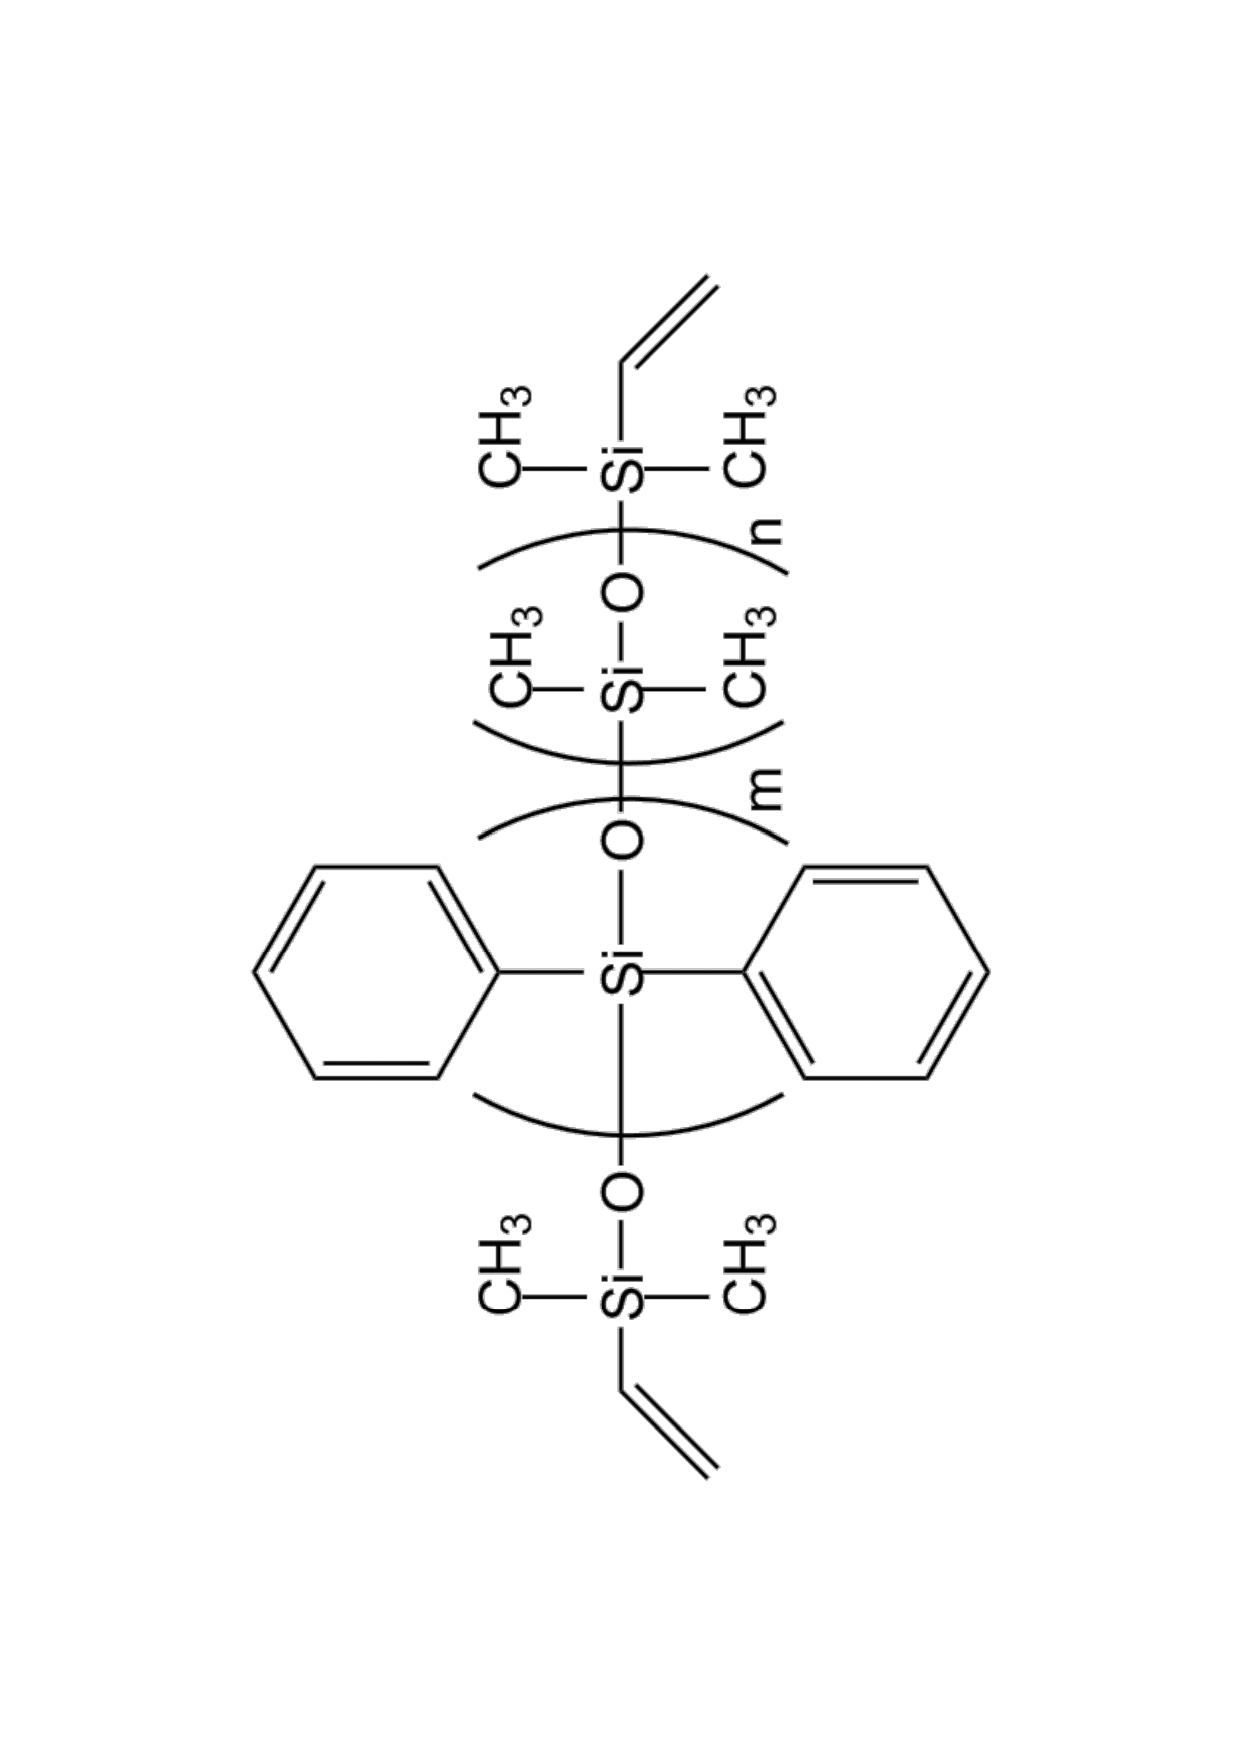
\includegraphics[angle=270,width=0.7\textwidth]{pics/ocf.pdf}
\caption{\label{pic:ocf}
A molecula of OCF-446 silicone fluid.
}
\end{figure}

There are two OCF-446 layers in the setup: one is between the PMT window and the cookie, another one is between the cookie and the window of the optical box. We can calculate the thickness of those layers based on the number of drops used. One drop is about $0.016$ g, density of the fluid is $1.04$ g/cm$^{3}$. Cookie area is $5.2$ cm times $15.8$ cm. I assume we use $2$ drops for the layer between the PMT and the cookie. This results into thickness of $0.0004$ cm. For the second layer we use $2$ drops to grease the cookie, and another $3$ drops to put in the middle of each PMT, which results into layer thickness of $0.00094$ cm.

\subsubsection*{Bialkali photocathode}

\begin{figure}[!h]
\centering
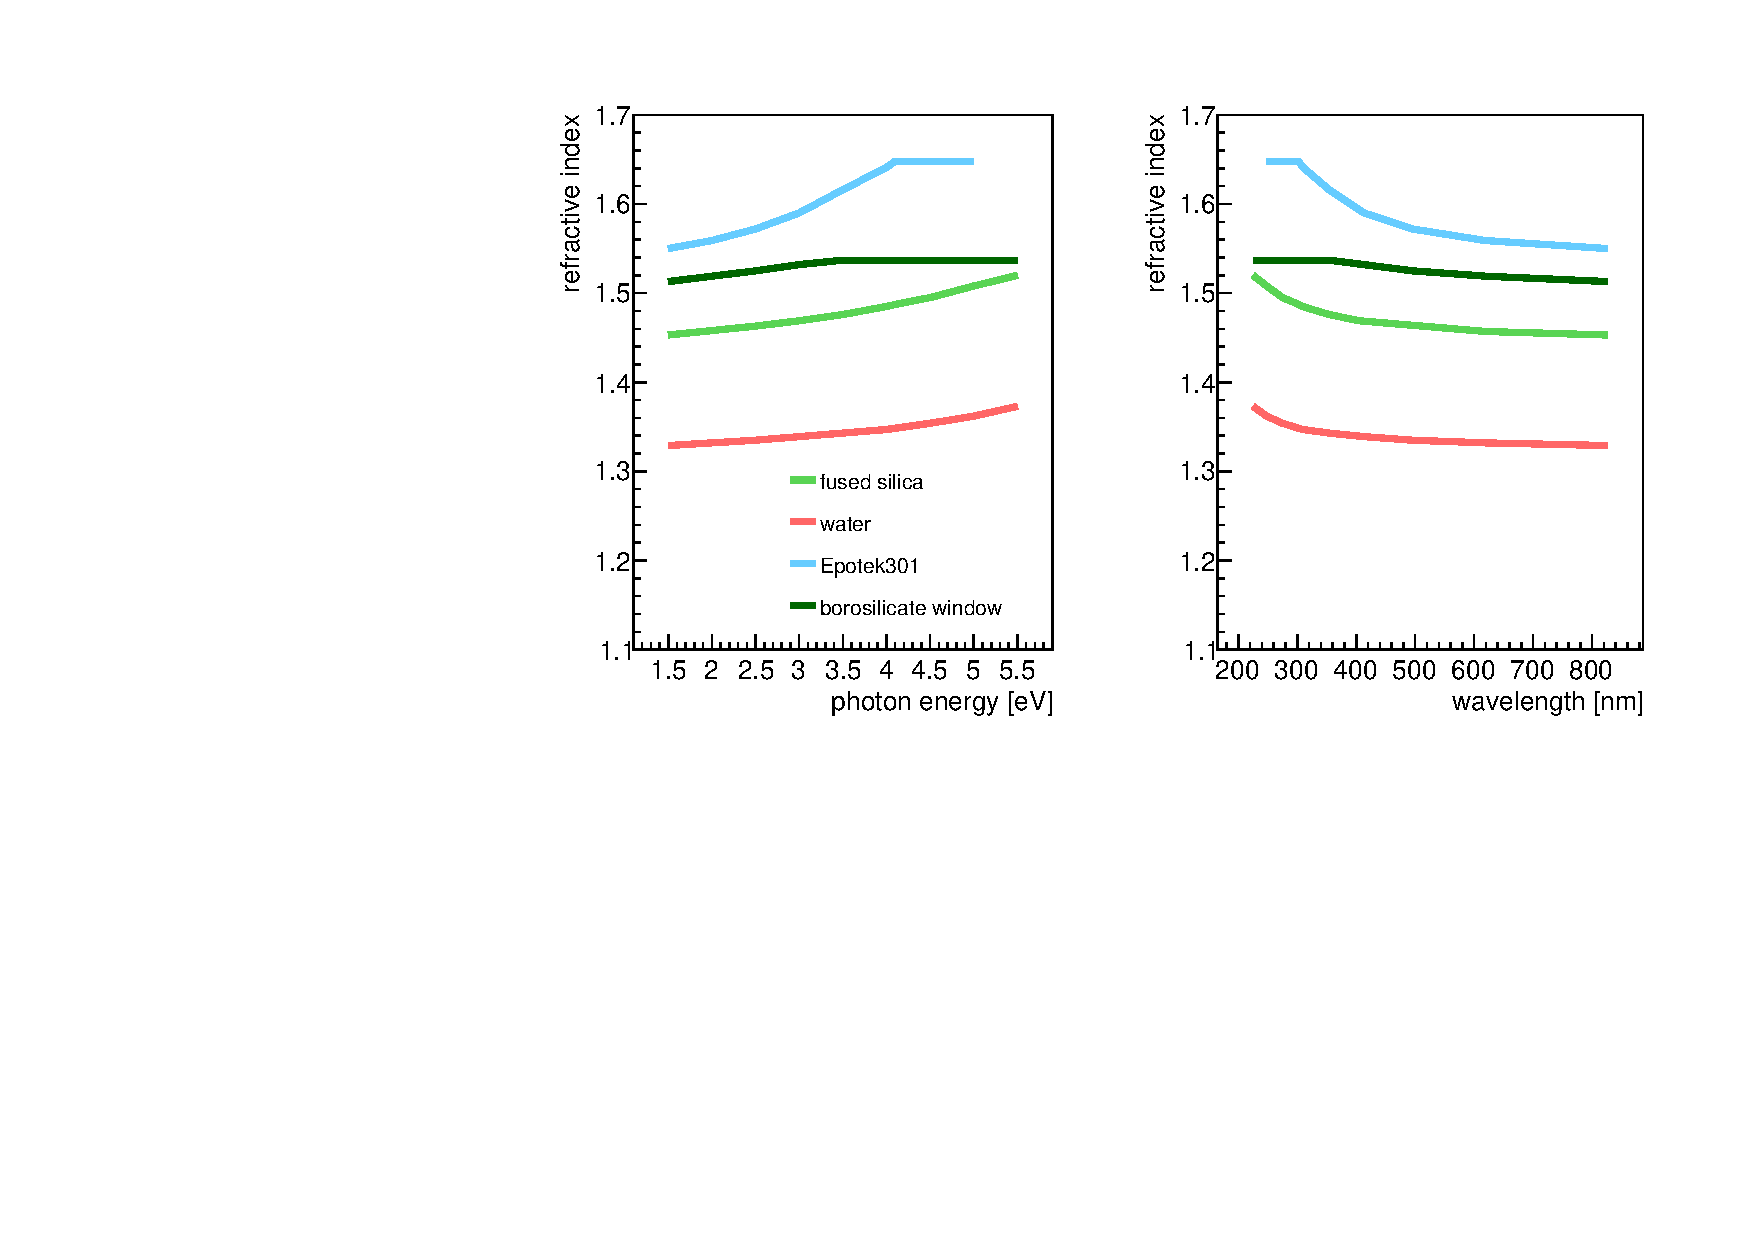
\includegraphics[angle=0,width=0.85\textwidth]{pics/refind.pdf} \\
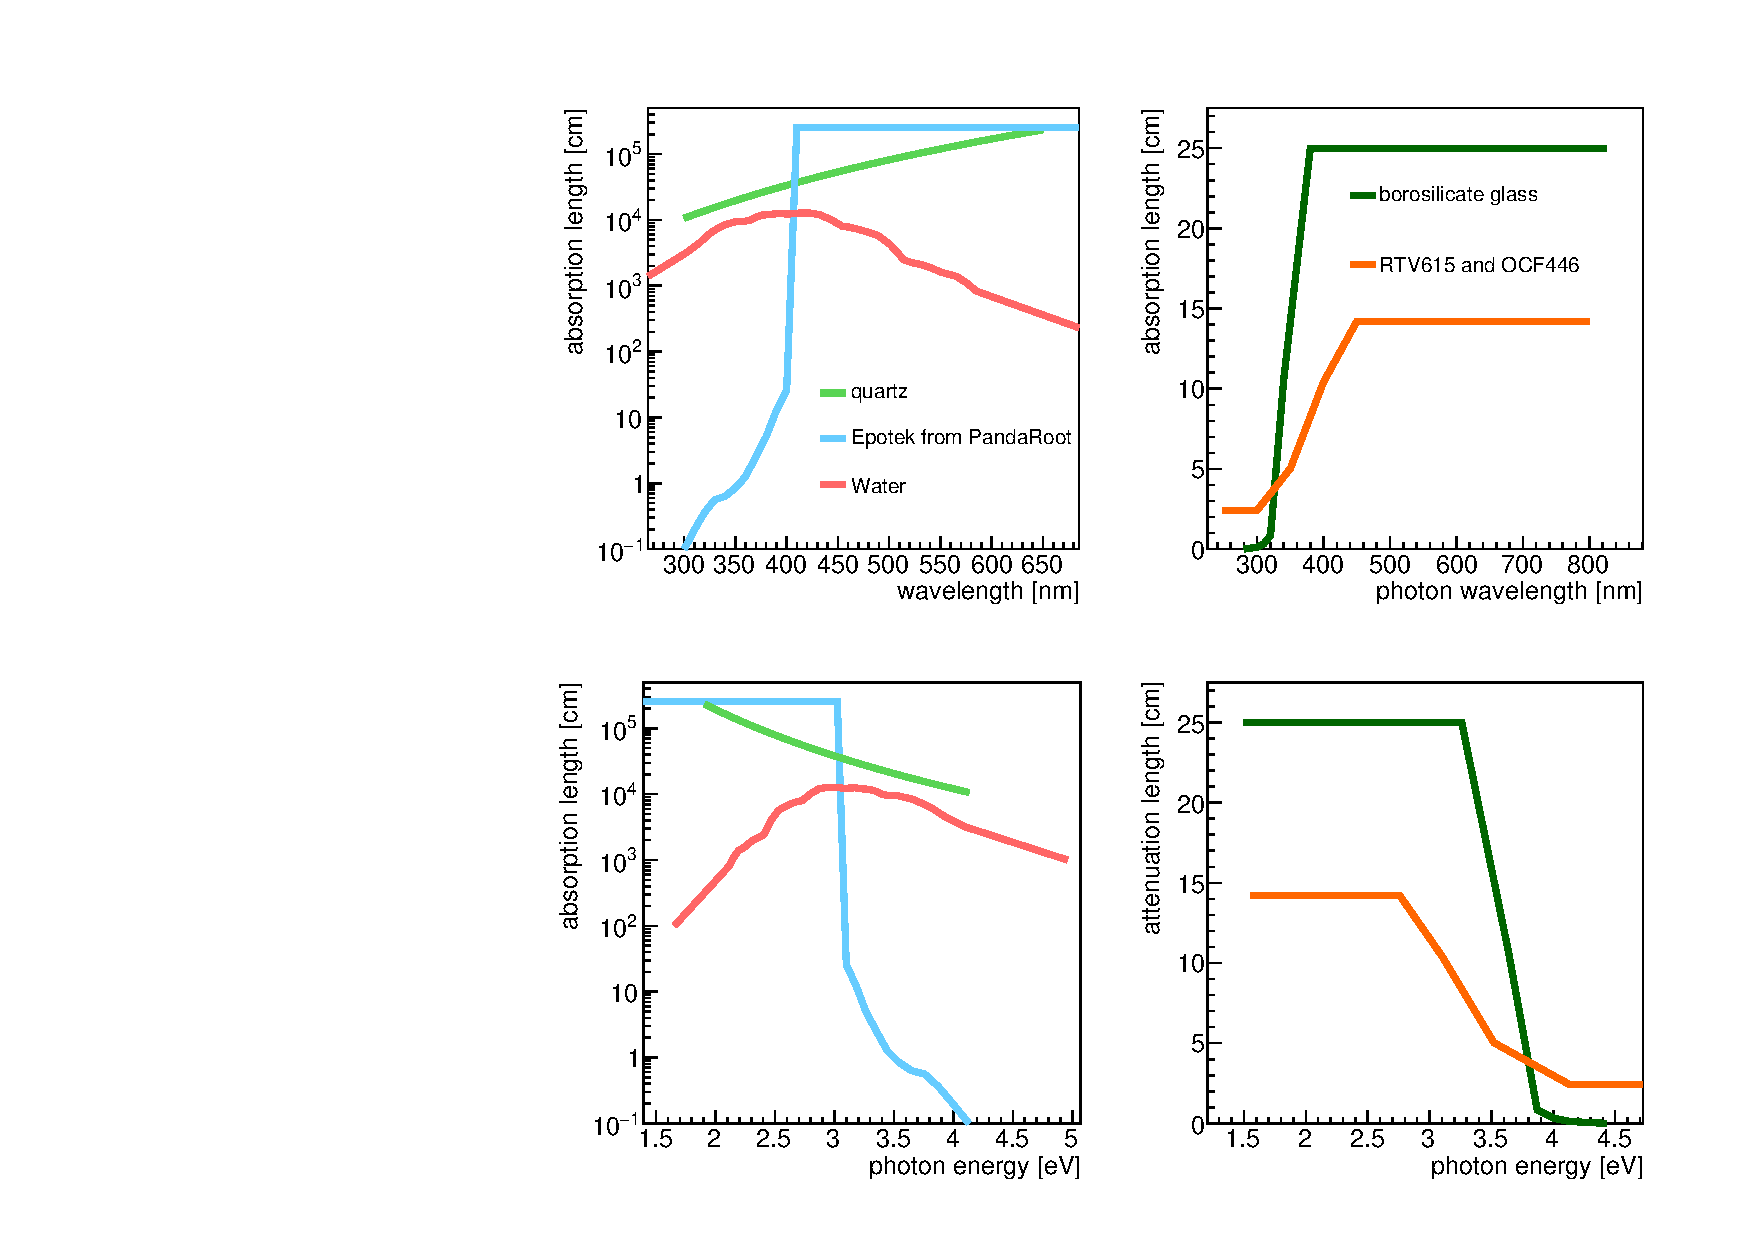
\includegraphics[angle=0,width=0.85\textwidth]{pics/ablen.pdf}
\caption{\label{pic:mat}
Cherenkov properties for some materials used in the simulation: refractive index (above) and absorption length (below).
}
\end{figure}

According to Ref~\cite{pcpaper}, photocathode is a thin layer of a multialkali (in our case bialkali) semiconducting alloy, which is evaporated onto the back side of the glass window during production. In the same paper we find, that it is quite difficult to extract properties of the photocathode itself. It can not be studied directly, as it is not chemically stable when exposed to air. Also, its properties might interefere with the birefringence, that is induced on the glass window by the mechanical stress due to the pressure difference (the interiour of the PMT is under vacuum). We use the simplified structure of the PMT: borosilicate window layer followed by a layer of photocathode with the thickness of $0.1$ cm (not realistic, but it does not matter, as our photons anyways get stopped in the photocathode). 

The quantum efficiency function defines properties of the photocathode, when the light is coming from air. For the case when instead air we have a medium with $n > 1$ (we have fused silica window with $n = 1.47$, in the paper they use scintillator with $n = 1.48$), authors~\cite{pcpaper} claim, that effective quantum efficiency is slightly increased compared to the one stated in data sheet. So in the simulation we will use the data sheet quantum efficiency as a conservative estimate. We use refractive index $n = 2.7$ to allow Geant4 do reflection/refraction on the PMT window -- photocathode interface. We use photocathode absorption length of $0.0001$ cm to stop Cherenkov photons and write out DIRC signal in the photocathode volume.

%Geant4 needs absorption length $\lambda$ as the following:

%\begin{equation}
%I = I_{0} \cdot e^{-x/\lambda},
%\end{equation}

%\noindent where $I_{0}$ is the incident intensity, $I$ -- transmitted intensity, $x$ -- thickness of the sample. Transmittance $T = I/I_{0}$ for the photocathode $T = 1 - A$, where $A$ -- absorption. In the paper~\cite{pcpaper} we see $A$ (410 nm) $= 0.44$ and $A$ (440 nm) $=0.41$, we take $A = 0.42$ and calculate $\lambda$ based on this assumption and the photocathode thickness of $x = 0.1$ cm. We get absorption length of $\lambda = 0.184$ cm. The refractive index of photocathode is $2.7$~\cite{pcpaper}. 

Fig.~\ref{pic:mat} show refractive indices and absorption lengths for different materials as a function of photon wavelength and energy.

\subsection{DIRC signal}

\begin{figure}[!h]
\centering
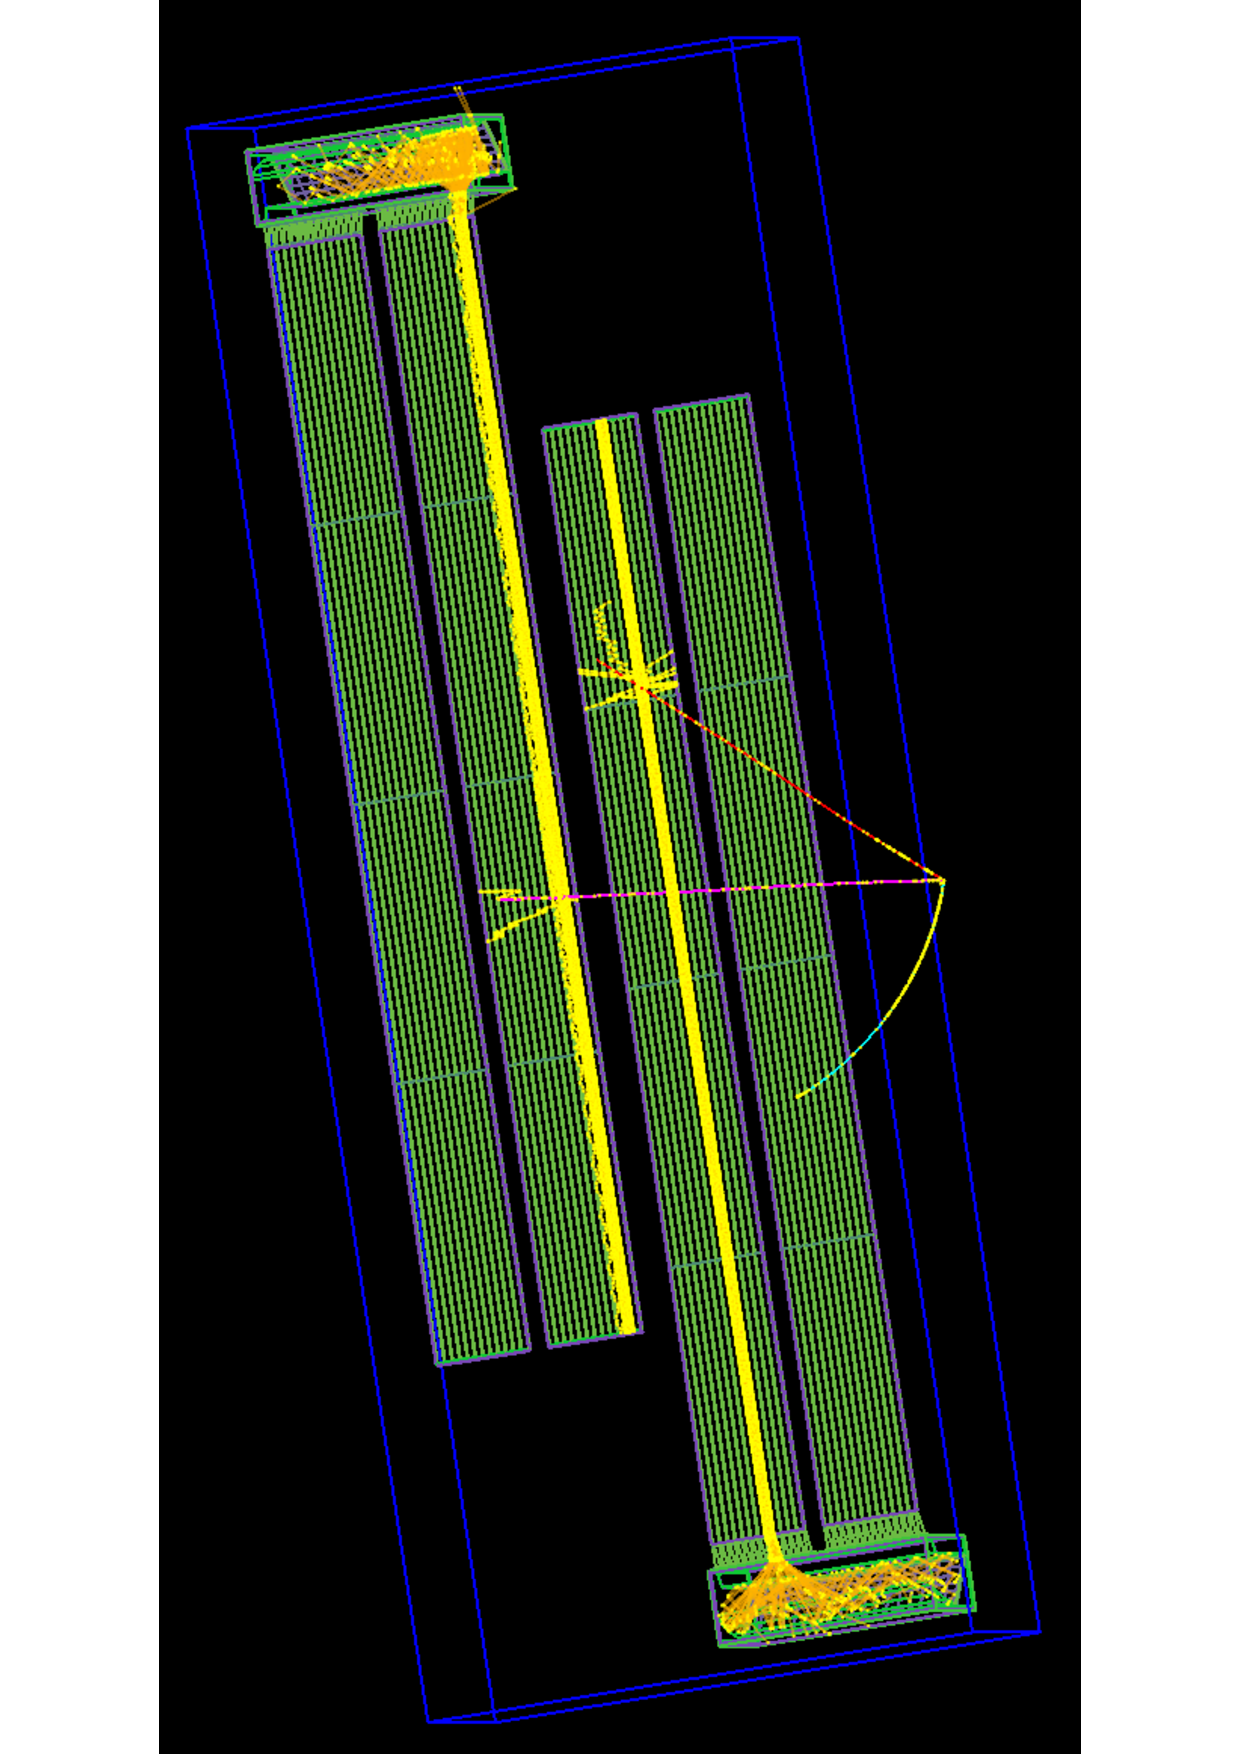
\includegraphics[angle=270,width=0.8\textwidth]{pics/eta2300decay.pdf}
\caption{\label{pic:eta2300}
An event showing the decay of $\eta_{2300}$ into a kaon (red track) and a pion (magenta track). 
%A pion is shown in magenta, a kaon is shown in red. 
%A proton is shown in cyan. 
The pion and proton create Cherenkov photons (yellow tracks) inside two different DIRC radiators. The photons are transported to the optical boxes, where a small fraction of them is imaged onto photodetection planes.
}
\end{figure}

Figure~\ref{pic:eta2300} shows a decay of $\eta_{2300}$. The final state pion is shown in magenta and hits the upper bar box. The final state kaon is shown in red and hits the lower bar box. Both charged particles produce Cherenkov photons (their trajectories are shown in yellow), that propagate inside individual radiators towards the optical boxes, where a small fraction of the initially created photons is detected. Hit patterns for this particular event are shown in Fig.~\ref{pic:hitpat1}. DIRC does not try to reconstruct the shape of the hit pattern, but use different methods to compare hit patterns $(x,y,z)$\footnote{It is convenient to use a separate coordinate system on the photodetection plane. There $x$ axis goes along the long rows of PMTs containing $18$ sensors each, and $y$ axis goes along the short PMT rows of $6$ sensors each.} to expectations for different particle hypotheses ($e, \mu, \pi, K, p$).

\begin{figure}[h]
\centering
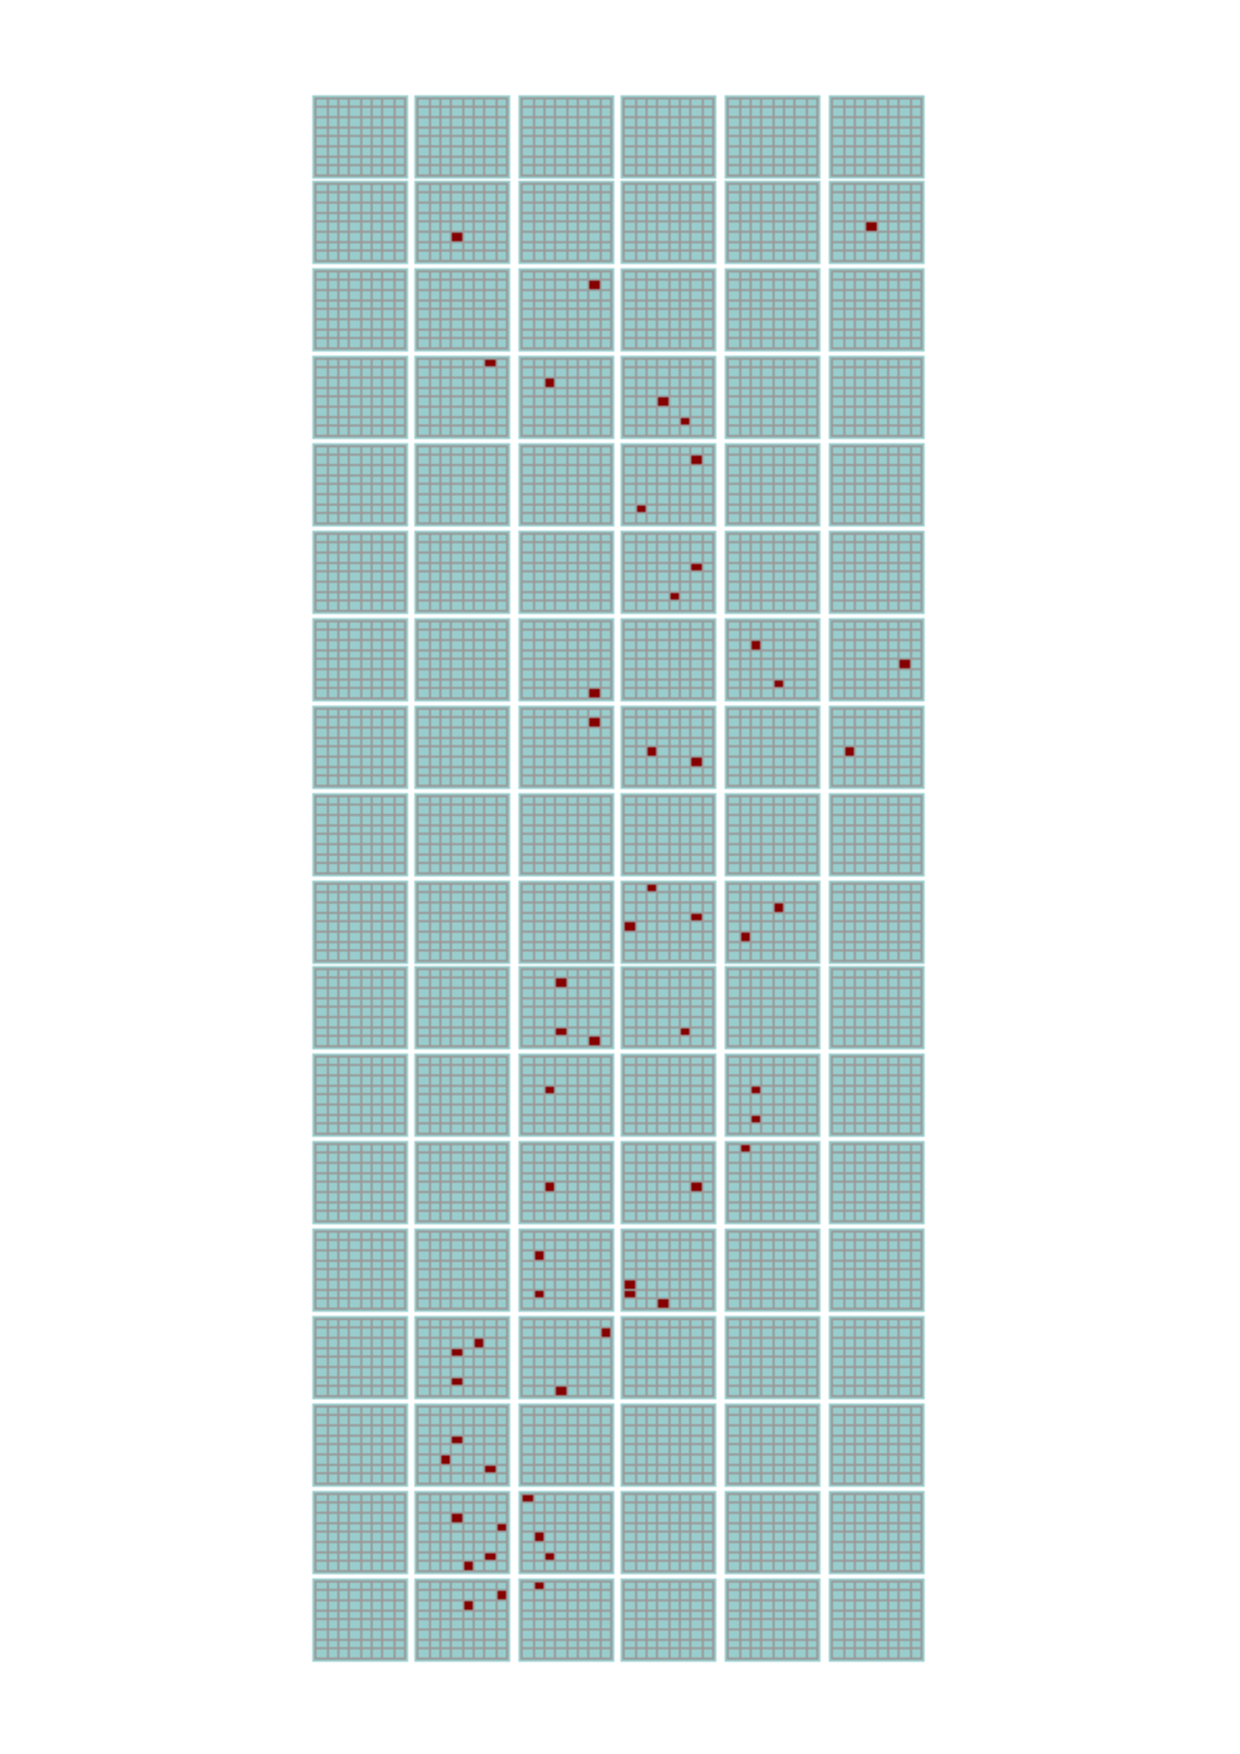
\includegraphics[angle=270,width=0.47\textwidth]{pics/pion_eta2300.pdf} \hspace{0.5cm} 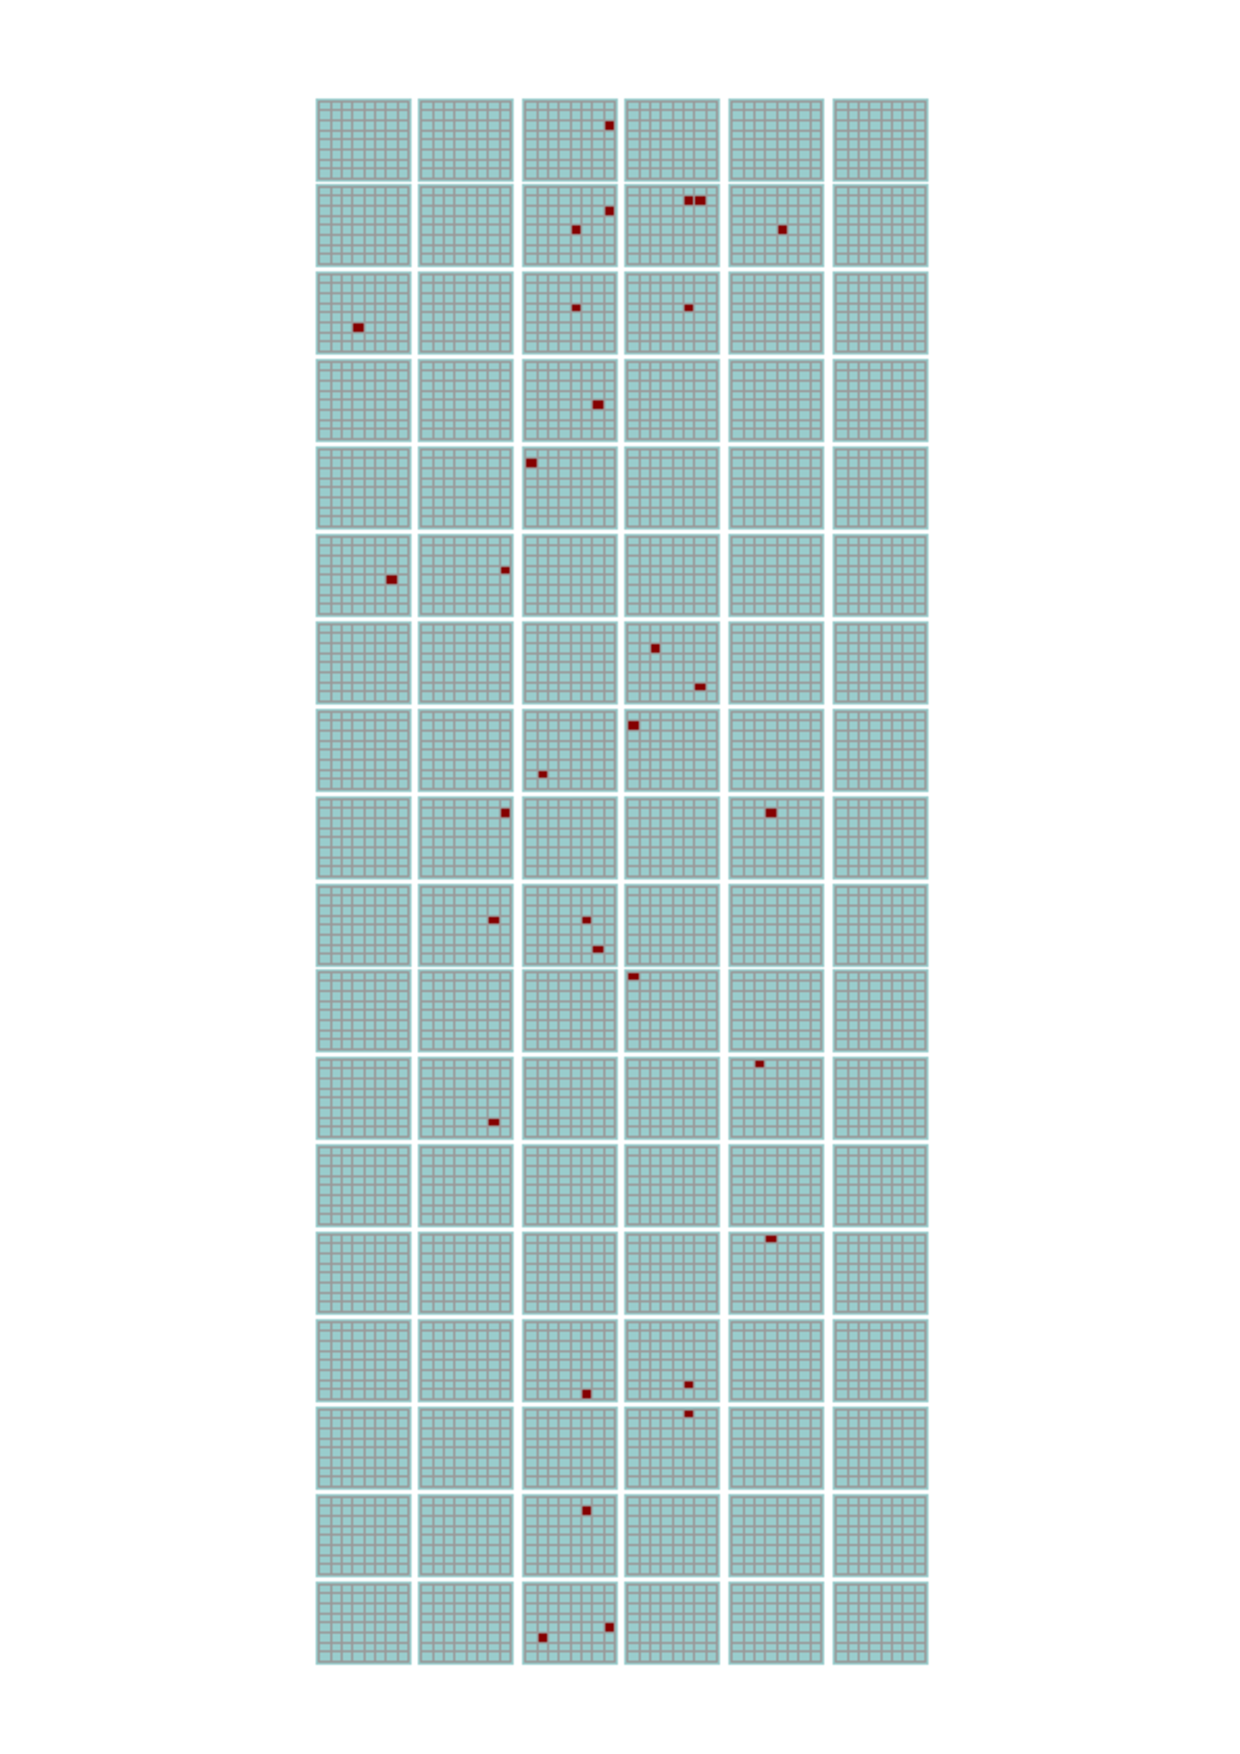
\includegraphics[angle=270,width=0.47\textwidth]{pics/kaon_eta2300.pdf}
\caption{\label{pic:hitpat1}
Hit patterns for the decay of $\eta_{2300}$ from Fig.~\ref{pic:eta2300}: for the pion (left) and kaon(right).
}
\end{figure}

DIRC measures $(x,y,t)$ of each Cherenkov photon. In $(x,y)$ the cumulative hit patterns looks like conic sections with reflections (see an interactive illustration \url{http://web-docs.gsi.de/~rdzhigad/www/research/hit-pattern-vs-theta-phi for detail}). In the coordinate space some parts overlap, but timing helps to separate them.
An example of the cumulative timing spectra for charged kaons with fixed momentum and direction is shown in Fig.~\ref{pic:time}. 

\begin{figure}[h]
\centering
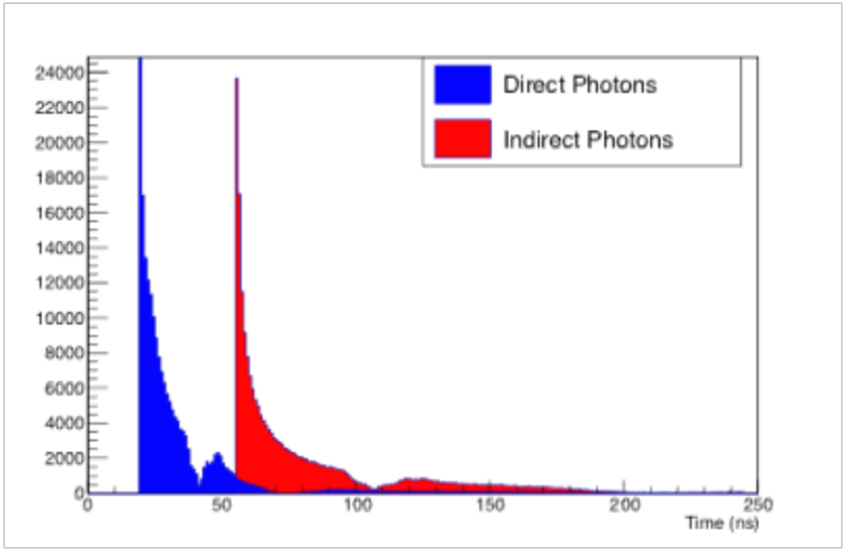
\includegraphics[angle=0,width=0.6\textwidth]{pics/time.pdf}
\caption{\label{pic:time}
An example of the cumulative timing signal for charged kaons with fixed momentum and direction. Blue distribution represents direct photons, which were transported inside the radiator straight to the optical box. Red distribution shows indirect photons, which first went to the mirror at the end of the radiator, and then towards the optical box. The spread of the timing signal for one track is tens of nanoseconds.
}
\end{figure}

An essential input for the DIRC reconstruction is the tracking information about the momentum of the charged particle and coordinate, where it hit the DIRC wall.

\begin{figure}[!h]
\centering
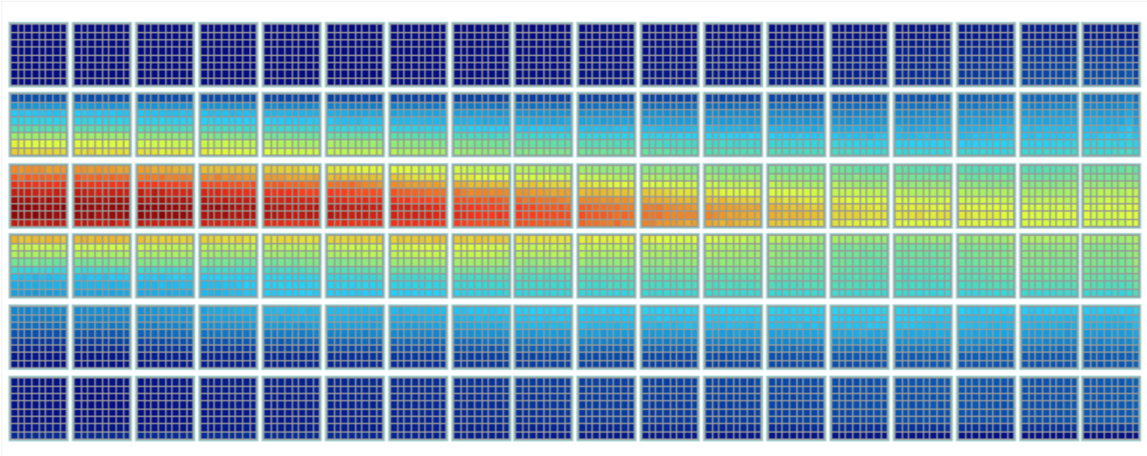
\includegraphics[angle=0,width=0.8\textwidth]{pics/phi1850.png}\\
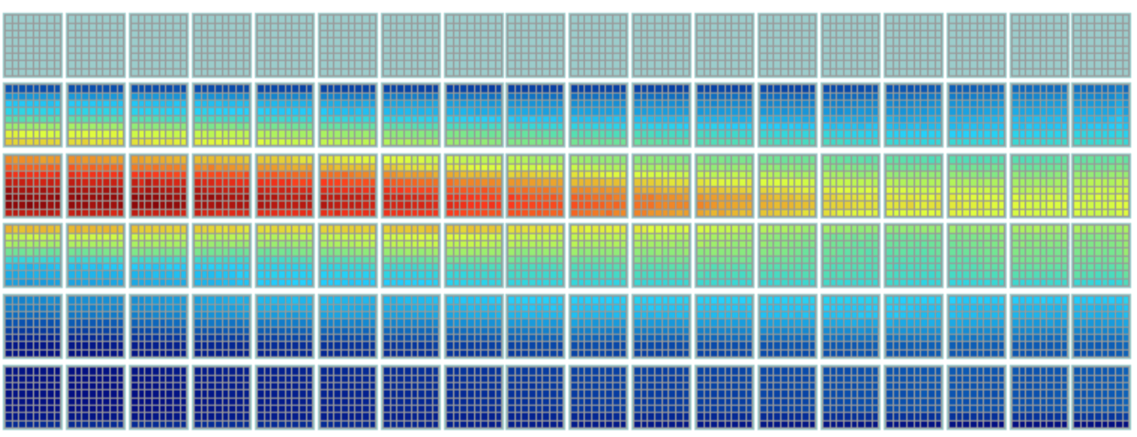
\includegraphics[width=0.8\textwidth]{pics/5rowsHP.png}
\caption{\label{pic:phi}
A cumulated kaon hit pattern for kaons coming from $\phi_{1850}$ decay. Cumulative kaon hit patterns for decays of $y_{2175}$, $h_{2600}$, $\Xi_{1820}$, $\eta'_{2300}$, and for the general background look very similar. The lower picture shows the removed upper row of photosensors. 
}
\end{figure}

To get a feeling about which parts of the photodetection plane are occupied more, and which less, we can have a look at the cumulative kaon occupancies originating from some relevant physics reactions or from general kaon background. Figure~\ref{pic:phi} shows an example for the cumulative kaon hit pattern for the decay of $phi_{1850}$. Kaon hit patterns for other reactions of interest and general background look very similar. The highest occupancy is around the third PMT row from the top. The hit pattern is not left-right symmetrical, as the left side of the optical box is closer to the beam line. The upper row of PMTs has the lowest occupancy. The simulation studies showed that removing this row does not impact to the detector performance in terms of photon yield and separation between pions and kaons (see Fig.~\ref{pic:5rows}).

\begin{figure}[!h]
\centering
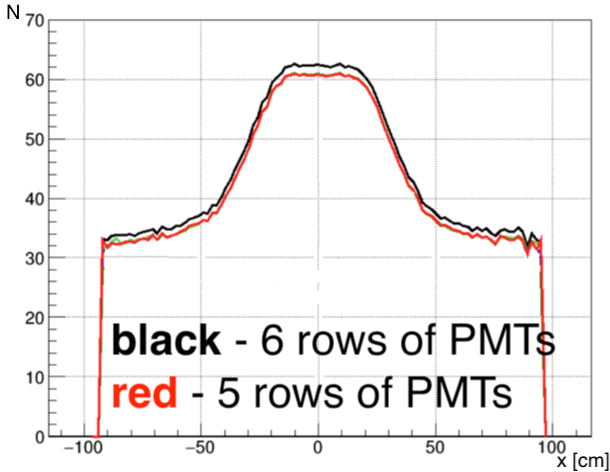
\includegraphics[angle=0,width=0.4\textwidth]{pics/5rows1.png} \hspace{0.5cm} 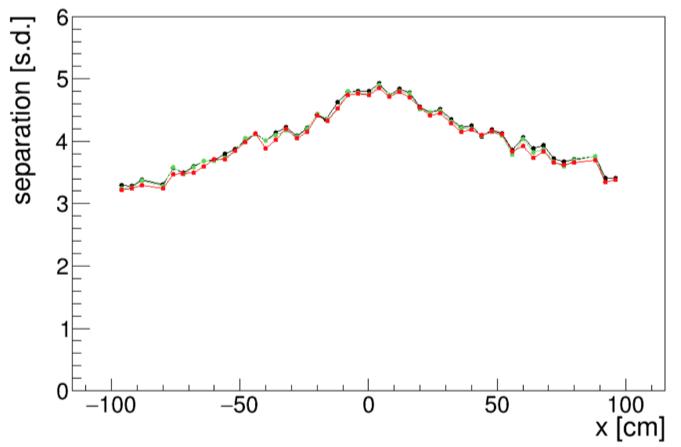
\includegraphics[width=0.45\textwidth]{pics/5rows2.png}
\caption{\label{pic:5rows}
Comparison of detector performance, when the photodetection plane is fully equipped with PMTs, and when the upper row is not equipped. The study was done for the radiator bar closest to the beam line. The left plot shows photon yield along the bar. The right plot shows separation between pions and kaons as a function of the charge particle position on the radiator bar. Black line shows fully equipped photodetection plane. Red line corresponds to the case when the upper row of photosensors was removed.
}
\end{figure}

\section{Reconstruction}
\subsection{Geometrical reconstruction}
\label{sec:gr}

\begin{figure}[!h]
\centering
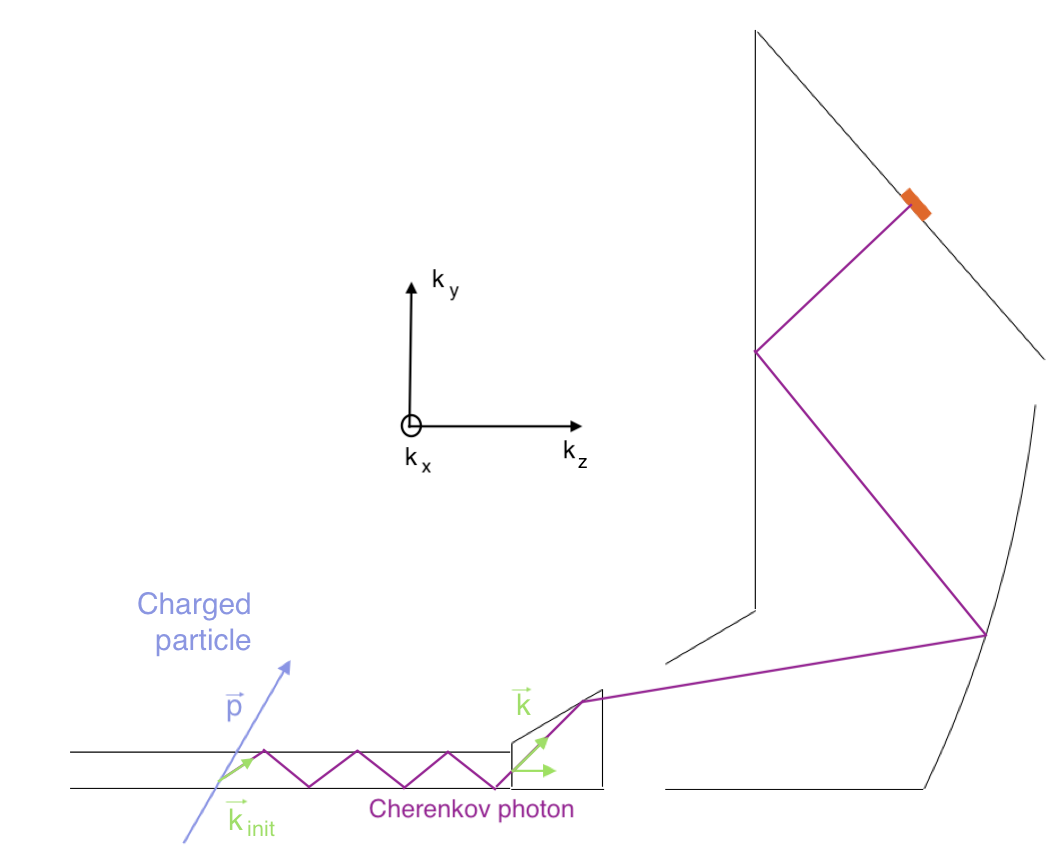
\includegraphics[width=0.8\textwidth]{pics/lut3.png}
\caption{\label{pic:lut1}
The concept of the geometrical reconstruction. One example Cherenkov photon is emitted by the charged particle. The photon direction $\vec k$ is an estimator of the initial photon direction $\vec k_{init}$ and is used to reconstruct $\theta_{C}$ for this photon (using charged paricle direction $\vec p$). The photon transportation is described in a depicted bar coordinate system, where axes are parallel to radiator sides. In that case reflection off a particular side results into a sign flip of the corresponding momentum component.
}
\end{figure}

The geometrical reconstruction is based on the BABAR DIRC approach. In this method, illustrated in Fig.~\ref{pic:lut1} the Cherenkov angle ($\theta_{C}$) is reconstructed for each detected photon individually based on the directions of the charged particle and the photon. The charged particle direction is identified by the tracking system. The photon direction is estimated using the spacial location of the radiator bar, where photon was produced, and that of the pixel, where the photon was detected.

This method is fast, because the mean photon direction for each pixel on the photodetection surface depends only on the detector geometry and can be simulated in advance and stored in a special map called ''look-up table''.

\begin{figure}[!h]
\centering
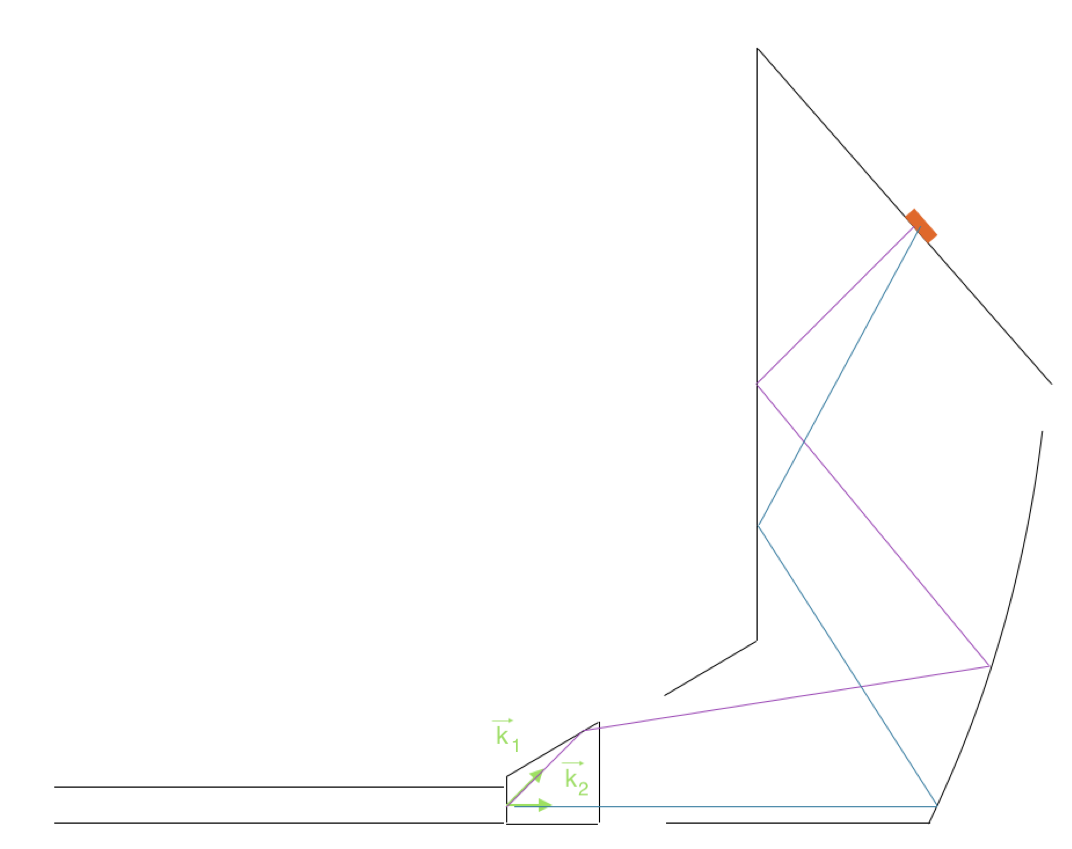
\includegraphics[width=0.8\textwidth]{pics/lut1.png}
\caption{\label{pic:lut2}
An illustration of one entry of the look-up table. Two photons wiht direction vectors $\vec k_{1}$ and $\vec k_{2}$ originate at the center of the bar, propagate throught the optical box, and end up in a given pixel. So the look-up table entry corresponding to the shown pixel contains $\vec k_{1}$ and $\vec k_{2}$ (and their propagation times).
}
\end{figure}

To produce a look-up table, one can set up a particle gun shooting single optical photons towards the optical box. The origin of the photons should be located in the middle of the bar end attached to the small wedge. Optical photons from the particle gun propagate throught the optical box and hit different pixels of the photodetection plane. The photons detected in the same pixel are grouped together, and their directions at the origin (vectors $\vec k_1$ and $\vec k_2$ in Fig.~\ref{pic:lut2}) are stored for the given pixel number in the look up table. The photon propagation time is stored too. For a particular radiator bar, one entry of the look-up table consist of a pixel number, a set of photon direction vectors and propagation times. A complete look-up table for the whole optical box includes 48 simulations with a particle gun located at the end of each radiator. A reasonable look-up table can be created using about 10 million single photons for one radiator bar.

The reconstruction procedure is the following. Each event (a charged particle of some particle type and momentum crosses the DIRC wall) yields a set of hit pixels (e.g. see Fig.~\ref{pic:hitpat1}). Each detected photon has a set of solutions for the $\vec k$ vectors stored in the ''look-up'' table (see Fig.~\ref{pic:lut2}). 
%A three-dimensional photon direction vector $\vec k$ (see Fig.~\ref{pic:lut1}) origins from the center of the bar end and defines the photon path through the optical box ending in the given pixel.  
Each $\vec k$ vector yields a set of $8$ solutions for the initial photon direction $\vec k_{init}$ (see Fig.~\ref{pic:lut1}), as the photon can effectively be reflected off any side inside the bar (see bar coordinate system depicted in Fig.~\ref{pic:lut1}).
Together with the track direction, each $\vec k_{init}$ gives one hypothesis for the reconstructed Cherenkov angle of the photon. Going through all the detected pixels, we plot the solutions for the reconstructed Cherenkov angle. Among these solutions there is always the correct one entering the signal peak in the distribution (see Fig.~\ref{pic:spr}). 
%Going through all the hit pixels for the particle track and collecting the reconstructed Cherenkov angles in a histogram gives a distribution peaking at the expected value of the Cherenkov angle. 
We can compare the peak position to the expectation, calculated based on the charged particle momentum and the mean refractive index of fused silica. The width of the obtained distribution represents the single photon Cherenkov angle resolution ($\sigma_{c}$, SPR).

\begin{figure}[!h]
\centering
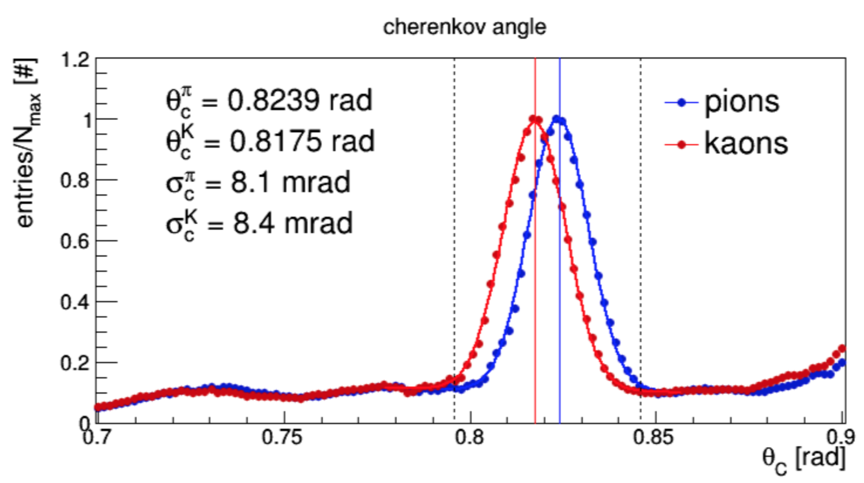
\includegraphics[width=0.8\textwidth]{pics/spr.png}
\caption{\label{pic:spr}
The distribution showing reconstructed Cherenkov angle per photon for kaons (red) and pions (blue) with momenta of $4$ GeV/c, and direction defined by $\theta = 4^{\circ}$ and $\phi = 90^{\circ}$. The vertical lines show expected values for the Cherenkov angles. 
%The values of the reconstructed Cherenkov angle and single photon Cherenkov angle resolution are shown.
}
\end{figure}

SPR is an useful quantity, as it can be measured experimentally and represents the detector accuracy, therefore, can be compared to other DIRCs.

The geometrical reconstruction uses timing information to cut out some solution for the Cherenkov angle and therefore reduce the combinatorial background.

The Cherenkov angle resolution for a track $\sigma_{\theta_{C}}$ is calculated as the following:

\begin{equation}
\sigma^{2}_{\theta_{C}} = \sigma^{2}_{tr} + \frac{\sigma^{2}_{C}}{N_{\gamma}},
\end{equation}

\noindent where $\sigma_{tr}$ is the tracking resolution, defined by the tracking system (is estimated to be at the order of $1$ mrad~\cite{tdr}), $\sigma_{\theta_{C}}$ -- single photon Cherenkov angle resolution, $N_{\gamma}$ -- number of detected photons per track (based on the simulation it is expected to be between 30 and 60, but that is very optimistic estimation).

\subsection{Extended log likelihood probability}

The DIRC measures the arrival times $t_{i}$ and positions $(x_{i}, y_{i})$ of the $N$ Cherenkov photons detected on the photodetection plane. The extended log likelihood probability for a given charged particle hypothesis $h$ 
%($\log\mathcal{L}$) for different particle hypotheses 
($h = e, \mu, \pi, K, p$) can be 
%calculated based on the reconstructed Cherenkov angle and the number of detected photons as the following
defined as~\cite{staric2}:

\begin{equation}
\log\mathcal{L}_{h} = \sum_{i=1}^{N} \log \Big( \frac{S_{h}(x_{i}, y_{i}, t_{i}) + B_{h}(x_{i}, y_{i}, t_{i})}{N} \Big) + \log P_{N}(N),
\label{eq:ll}
\end{equation}

\noindent where $S_{h} (x_{i}, y_{i}, t_{i})$ is the signal distribution for the hypothesis $h$ (in our case it is reconstructed Cherenkov angle) and $B(x_{i}, y_{i}, t_{i})$ is the distribution of background, and $N_{e} = N_{h} + N_{B}$ is the expected number of detected photons, being a sum of the expected number of signal photons $N_{h}$ for hypothesis $h$ and the expected number of background photons, $N_{B}$. The second term in Eq.~\ref{eq:ll} is the Poisson probability to obrain $N$ photons if the mean is $N_{e}$.
%$P_{N}(N)$ is the probability to get the measured number of Cherenkov photons for this hypothesis based on the distribution of the number of expected photons.

Distributions $S_{h} (x_{i}, y_{i}, t_{i})$ and $B(x_{i}, y_{i}, t_{i})$ in Eq.~\ref{eq:ll} are normalized in the following way:

\begin{equation}
\sum_{j=1}^{n_{ch}} \int_{0}^{t_{m}} S_{h}(x_{j}, y_{j}, t) dt = N_{h}
\label{eq:norm1}
\end{equation}

\begin{equation}
\sum_{j=1}^{n_{ch}} \int_{0}^{t_{m}} B(x_{j}, y_{j}, t) dt = N_{B}
\label{eq:norm2}
\end{equation}

\noindent where the sum runs over all channels $n_{ch}$ of the photon detector array, $(x_{j}, y_{j})$ being detector coordinates, and the integration is performed over the full range $t_{m}$ of the time-of-arrival measurement.

\begin{figure}[!h]
\centering
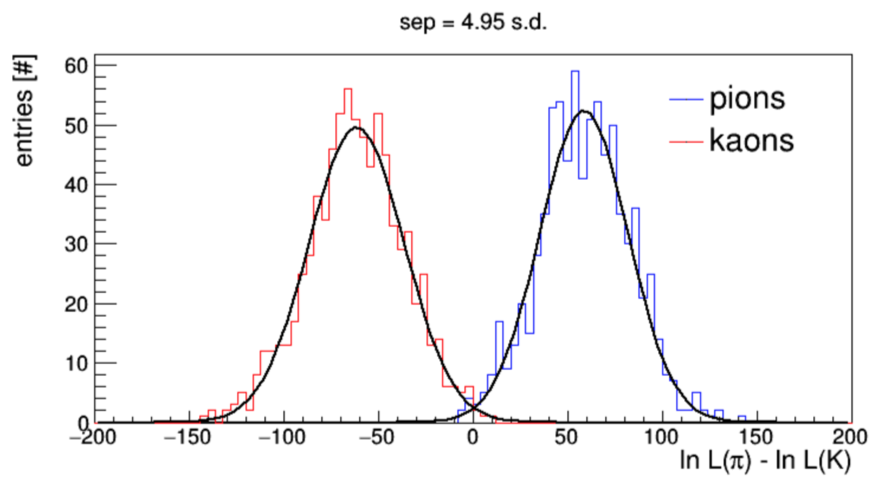
\includegraphics[width=0.8\textwidth]{pics/sepLUT.png}
\caption{\label{pic:sepLUT}
The separation between kaons (red) and pions (blue) with momenta of $4$ GeV/c, and direction defined by $\theta = 4^{\circ}$ and $\phi = 90^{\circ}$ is 4.95 s.d.
}
\end{figure}

Separation between kaons and pions can be calculated based on the difference in log likelihoods (see Fig.~\ref{pic:sepLUT}).

\subsection{Time Imaging reconstruction}
\label{sec:ti}

The ring image of the GlueX DIRC is a complicated pattern in $(x, y, t)$ space, which besides Cherenkov angle depends strongly on the particle impact position and the particle direction with respect to the sides of the quartz bar. For the forward GlueX DIRC geometry, the charged particle direction with respect to the sides of the DIRC radiators correlates with the position where the charged particle hit the DIRC wall. We can draw conclusion about the particle type just directly comparing the given hit pattern in terms of $(x, y, t)$ to the ones for different particle species and constructing extended log likelihoods, discussed in the previous section. To do so, we need to fix the momentum and direction of the particle, so that the comparison is between various particle types and the kinematical variables are the same.

\begin{figure}[!h]
\centering
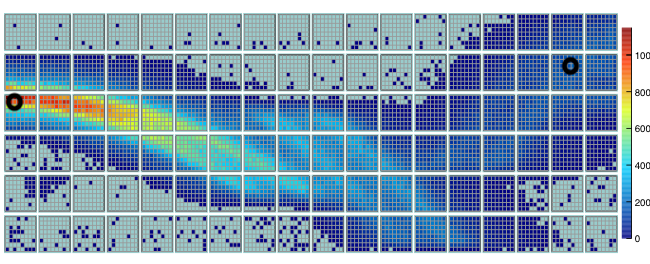
\includegraphics[width=0.55\textwidth]{pics/kaonsTI.png} \hspace{0.05\textwidth} 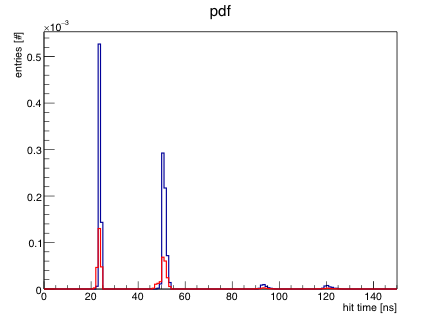
\includegraphics[width=0.35\textwidth]{pics/LeftPix.png} \\
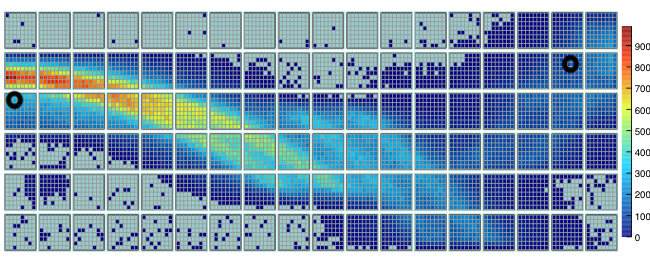
\includegraphics[width=0.55\textwidth]{pics/pionsTI.png} \hspace{0.05\textwidth} 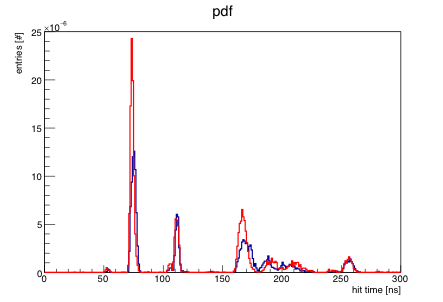
\includegraphics[width=0.35\textwidth]{pics/rightPix.png} 
\caption{\label{pic:hitpatKpi}
Hit pattern for kaons (upper left) and pions (bottom left) with momentum of $2$ GeV/c, and direction defined by $\theta = 1.2^{\circ}$ and $\phi = 90^{\circ}$. Black circles mark two pixels, for which timing spectra are shown on the right. The upper timing spectrum is for the left circled pixel, the lower -- for the right circled pixel. Red color correspond to pions, blue -- to kaons.
}
\end{figure}
 
Figure~\ref{pic:hitpatKpi} illustrates the principle of the time imaging  algorithm. The left column show reference $(x, y)$ hit patterns for pions and kaons with momentum of $2$ GeV/c and same kinematical parameters. The upper hit pattern (kaons) is clearly shifted downward by about one size of a PMT with respect to the lower one (pions). The black circles mark two pixels on the photodetection plane, for which timing spectra are shown on the right. The upper right plot shows time distribution for the left circled pixel, and the lower right plot shows time distribution for the right circled pixel. The red color corresponds to pions, and blue -- to kaons. The timing spectra are normalized as Eq.~\ref{eq:norm1}.

To reconstruct an event (e.g. see Fig.~\ref{pic:hitpat1}) means to compare timing spectra in all hit pixels with the reference spectra for pions and for kaons, construct extended log likelihoods and derive a quantitative measure of the particle to be a pion or a kaon. This idea can be easily extended for more particle species including protons, muons, and electrons. The reference timing spectra can be either simulated or calculated analytically~\cite{staric2}~\cite{staric3}. Currently, we use simulated reference timing spectra.

The time imaging reconstruction method is sensitive to the single photon timing resolution. Indeed, the timing information is used here directly, unlike for the geometrical algorithm, where only coarse timing information is needed to cut out some solutions of the reconstructed Cherenkov angle. Figure~\ref{pic:sepTI2} shows separation between kaons and pions for two values of the single photon timing resolutions. The single photon timing resolution of 1 ns is approximately the value we are getting experimentally with the PMTs and the electronics boards. It is not enough to separate between kaons and pions using time imaging method.

\begin{figure}[!h]
\centering
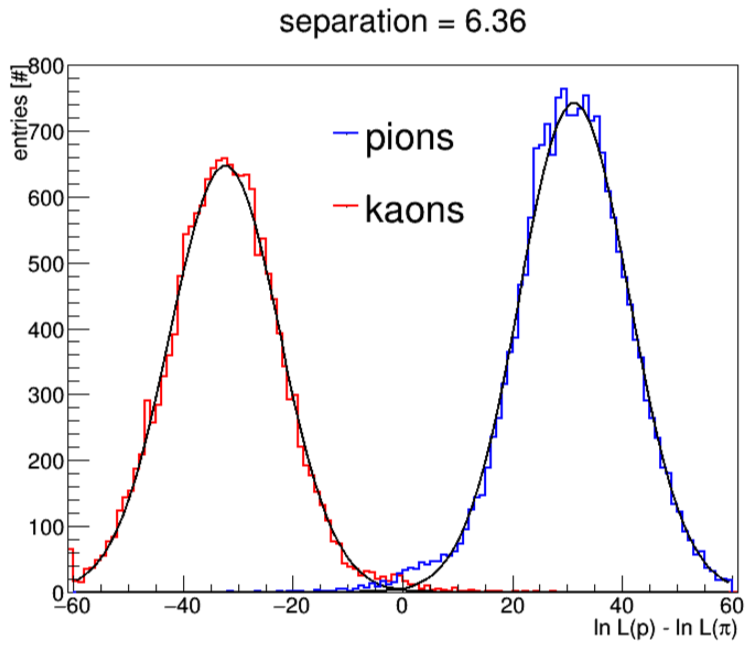
\includegraphics[width=0.43\textwidth]{pics/sepTI300.png} \hspace{0.5cm} 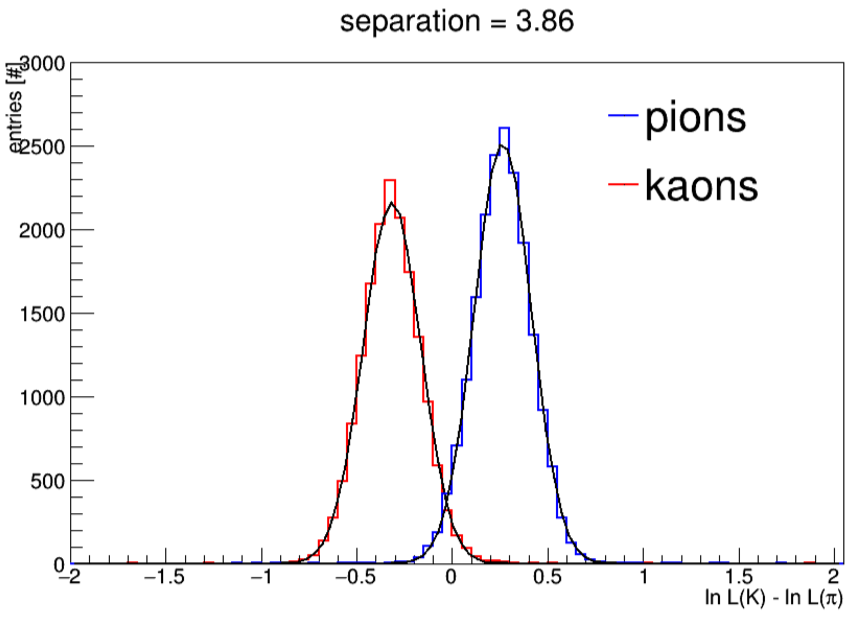
\includegraphics[width=0.52\textwidth]{pics/sepTI1000.png}
\caption{\label{pic:sepTI2}
The separation between kaons (red) and pions (blue) with momenta of $4$ GeV/c, and direction defined by $\theta = 4^{\circ}$ and $\phi = 90^{\circ}$. The left plot corresponds to the timing resolution of $300$ ps and it shows 6.4 s.d separation between kaons and pions. The right plot corresponds to $1$ ns timing resolution and it shows 3.9 s.d. separation between kaons and pions. \newline \footnotesize{Different $x$ axis scales are an artefact of the development work: the difference is due to the fact that the log likelihood for the left plot did not have $N$ detected photons in the denominator, and the right plot did have. The number of detected photons for high momentum particles is the same for pions and kaons, therefore this issue does not influence the performance for the given case. }
}
\end{figure}

\subsection{KDE-based reconstruction}

\subsection{Comparison of the performance}
 
\newpage
\begin{thebibliography}{1}
\bibitem{dirc} F.~Barbosa et al., ''The GlueX DIRC detector'', NIM \textbf{A} 876 (2017) 69.
\bibitem{gluex1} GlueX Collaboration, Mapping the Spectrum of Light Quark Mesons and Gluonic Excitations with Linearly Polarized Photons, Jefferson Lab PAC 30 Proposal, 2006.
\bibitem{gluex2} A.~AlekSejevs et al., GlueX Collaboration, \url{arXiv:1305.1523}.
\bibitem{gluex3} M.~Dugger et al., GlueX Collaboration, \url{arXiv:1408.0215}. 
\bibitem{bdirc1} I.~ Adam et al., NIM \textbf{A} 538 (2005) 235.
\bibitem{fdirc} B.~Dey et al., NIM \textbf{A} 775 (2015) 112.
\bibitem{scalar} H.~Bennet, J.~Elson, and J.~Bennet ``Scattering from optical surfaces'' Vol. 7. Applied Optics and Optical Engineering. Academic Press New York, 1979.
\bibitem{roughness} J.~Cohen-Tanugi et al., ``Optical properties of the DIRC fused silica Cherenkov radiator'', NIM \textbf{A} 515 (2003) 680. 
\bibitem{Epotek} Epoxy Technology, Inc. 14 Fortune Drive Billerica, MA 01821.
\bibitem{pcpaper} D.~Motta, S.~Sch{\"o}nert ''Optical properties of bialkali photocathodes'' NIM \textbf{A} 539 (2005) 217. 
\bibitem{water} A.~Morel ''Optical properties of Pure Water and Pure Sea Water'', Academic Press, 1974.
\bibitem{water2} R.~R{\"o}ttgers, ''Measurements of inherent optical properties of pure water'', Technical note, GKSS Forschungszentrum in der Helmholtz Gemeindschaft.
\bibitem{tdr} GlueX Collaboration, ''GlueX DIRC Technical Design Report'', 2015 
\bibitem{staric2} M.~Staric et al., ''Pattern recognition for the time-of-propagation counter'', NIM \textbf{A} 639 (2011) 252
\bibitem{staric3} M.~Static et al., ''Likelihood analysis of patterns in a time-of-propagation (TOP) counter'', NIM \textbf{A} 595 (2008) 252.
\end{thebibliography}

\end{document}

